\documentclass[conference,compsoc]{IEEEtran}
% IEEE S&P 2027 submission format: IEEEtran 1.8b, conference + compsoc, US letter, no margin or font changes.
\usepackage[nocompress]{cite}
\usepackage{amsmath,amssymb}
\usepackage{booktabs}
\usepackage{float}
\usepackage{graphicx}
\usepackage{array}
\usepackage[hyphens]{url}
\usepackage{xcolor}
\usepackage[hidelinks]{hyperref}
\newcommand{\artifactlink}[1]{\texorpdfstring{\href{https://github.com/submissionrepo/too-big-to-vote-on-artifact}{\textcolor{blue}{#1}}}{#1}}
% generated by make_numbers.py; do not edit by hand
\newcommand{\nResolved}{5,004}
\newcommand{\nVotes}{2,345,534}
\newcommand{\nVotesAll}{2,374,174}
\newcommand{\nPolymarket}{4,810}
\newcommand{\nGovernance}{26}
\newcommand{\nEraA}{886}
\newcommand{\nEraB}{4,118}
\newcommand{\nEraAPolymarket}{799}
\newcommand{\nEraBPolymarket}{4,011}
\newcommand{\nContested}{169}
\newcommand{\nContestedEraA}{80}
\newcommand{\nContestedEraB}{89}
\newcommand{\nPivotal}{57}
\newcommand{\nPivotalEraA}{29}
\newcommand{\nPivotalEraB}{28}
\newcommand{\nKleThreeEraB}{88}
\newcommand{\nTooEarlyWinsContested}{65}
\newcommand{\winMinEraA}{0.502}
\newcommand{\winMinEraB}{0.651}
\newcommand{\winMedEraA}{0.872}
\newcommand{\winMedEraB}{0.962}
\newcommand{\winPTenEraA}{0.625}
\newcommand{\winPTenEraB}{0.892}
\newcommand{\nEraAUnderSixtyFive}{103}
\newcommand{\nEraBWithinTwo}{4}
\newcommand{\nEraBWithinTen}{46}
\newcommand{\nPivotalYesNo}{29}
\newcommand{\nPivotalTooEarly}{28}
\newcommand{\partMedEraA}{0.885}
\newcommand{\partMedEraB}{0.964}
\newcommand{\partMedEraBPct}{96.4}
\newcommand{\votersMedEraA}{190}
\newcommand{\votersMedEraB}{518}
\newcommand{\nRolledEraA}{25}
\newcommand{\nRolledEraB}{40}
\newcommand{\nRepeatRollsEraA}{2}
\newcommand{\nRepeatRollsEraB}{14}
\newcommand{\nDeleted}{1}
\newcommand{\nTwentyTwentyFiveBeforeChange}{347}
\newcommand{\nTwentyTwentyFiveUnderSixtyFive}{11}
\newcommand{\minorityPTwentyFive}{0.138}
\newcommand{\minorityMedian}{0.188}
\newcommand{\minorityPSeventyFive}{0.256}
\newcommand{\slackPTen}{0.030}
\newcommand{\slackMedian}{0.142}
\newcommand{\topSupporterMedian}{0.092}
\newcommand{\topSupporterMax}{0.293}
\newcommand{\stakeNow}{19,357,995}
\newcommand{\topOnePct}{16.9}
\newcommand{\topFourPct}{37.12}
\newcommand{\topTenPct}{59.8}
\newcommand{\kStall}{4}
\newcommand{\kSixtyFive}{13}
\newcommand{\maxSingleEver}{32.0}
\newcommand{\nRoleChecked}{162}
\newcommand{\nManagedPayout}{14}
\newcommand{\managedSince}{October 2025}
\newcommand{\nPayoutVotes}{625}
\newcommand{\nBondOnlyVotes}{4,185}
\newcommand{\nPayoutVotesEraB}{480}
\newcommand{\payoutVotesPct}{13}
\newcommand{\nPmQuestionsVoted}{4,185}
\newcommand{\nPmQuestionsOneVote}{3,591}
\newcommand{\nContestedPm}{165}
\newcommand{\nPayoutContested}{51}
\newcommand{\nPayoutContestedEraA}{23}
\newcommand{\nPayoutContestedEraB}{28}
\newcommand{\nPayoutPivotal}{12}
\newcommand{\nPayoutPivotalEraA}{6}
\newcommand{\nPayoutPivotalEraB}{6}
\newcommand{\nPayoutPivotalYesNo}{7}
\newcommand{\nPayoutPivotalTooEarly}{5}
\newcommand{\nPayoutKleThreeEraB}{28}
\newcommand{\nPayoutTooEarlyWins}{15}
\newcommand{\payMinorityMedian}{0.157}
\newcommand{\paySlackMedian}{0.175}
\newcommand{\paySlackPTen}{0.075}
\newcommand{\payTopSupporterMedian}{0.094}
\newcommand{\payTopSupporterMax}{0.292}
\newcommand{\nNonPm}{194}
\newcommand{\nNonPmGov}{26}
\newcommand{\nNonPmAcross}{143}
\newcommand{\nNonPmYesNo}{17}
\newcommand{\nNonPmAssert}{8}
\newcommand{\nNonPmContested}{4}
\newcommand{\marchStake}{22,845,749}
\newcommand{\marchYes}{12,292,521}
\newcommand{\marchTooEarly}{8,706,371}
\newcommand{\marchNo}{1,144}
\newcommand{\marchAbstain}{1,845,686}
\newcommand{\marchVoters}{514}
\newcommand{\marchYesPct}{53.8}
\newcommand{\marchYesVotesPct}{58.5}
\newcommand{\marchYesVotesBps}{5853}
\newcommand{\marchTooEarlyPct}{38.1}
\newcommand{\marchAbstainPct}{8.1}
\newcommand{\marchParticipationPct}{92}
\newcommand{\marchWhale}{5,083,491}
\newcommand{\marchMargin}{869,647}
\newcommand{\marchMarginPct}{3.81}
\newcommand{\marchHF}{31.56}
\newcommand{\marchAlpha}{22.25}
\newcommand{\marchThetaMinusHF}{18.44}
\newcommand{\marchHT}{38.11}
\newcommand{\marchYesMinusWhalePct}{31.6}
\newcommand{\marchNeeded}{4,213,845}
\newcommand{\marchNeededSixtyFive}{7,640,707}
\newcommand{\marchShortSixtyFive}{2,557,216}
\newcommand{\marchNeededVotesCast}{3,291,002}
\newcommand{\marchStallStakedFifty}{11,422,874}
\newcommand{\marchStallStakedSixtyFive}{7,996,012}
\newcommand{\marchStallVotesSixtyFive}{15,992,024}
\newcommand{\marchPool}{10,553}
\newcommand{\marchWhaleGain}{4,364}
\newcommand{\marchWhaleShareOfWinners}{41.4}
\newcommand{\marchFirstYesPct}{50.2}
\newcommand{\marchFirstMarginPct}{0.19}
\newcommand{\portEvents}{819}
\newcommand{\portMatchedA}{396}
\newcommand{\portMatchedB}{397}
\newcommand{\portMismatched}{0}
\newcommand{\marchRedeemed}{1,129,633}
\newcommand{\marchRedeemedM}{1.13}
\newcommand{\marchRedeemers}{960}
\newcommand{\marchRedemptions}{1,097}
\newcommand{\marchTopRedeemer}{169,664}
\newcommand{\marchTopFiveSharePct}{44.6}
\newcommand{\marchUnredeemed}{17,735}
\newcommand{\marchVolumeM}{7.08}
\newcommand{\umaPriceMarch}{1.41}
\newcommand{\umaPriceNow}{0.45}
\newcommand{\marchStakeUsdM}{32.2}
\newcommand{\marchWhaleUsdM}{7.2}
\newcommand{\stakeNowUsdM}{8.6}
\newcommand{\marchTwap}{0.17}
\newcommand{\marchDisputeBuyShares}{486,583}
\newcommand{\marchDisputeBuyCost}{104,749}
\newcommand{\marchDisputeBuyWallets}{260}
\newcommand{\marchPostRevealShares}{177,792}
\newcommand{\marchPostRevealCost}{72,566}
\newcommand{\marchPostRevealWallets}{65}
\newcommand{\marchPostRevealLowCents}{16}
\newcommand{\marchPostRevealHighCents}{34}
\newcommand{\marchPostRevealMaxCents}{98}
\newcommand{\captureReqSixtyFiveMarch}{33.44}
\newcommand{\windowEmptyAt}{25.75}
\newcommand{\topFourShareExact}{37.12}
\newcommand{\realizedCaptureVotes}{30.84}
\newcommand{\realizedCaptureStaked}{33.44}
\newcommand{\laplacianGridPoints}{4,587}
\newcommand{\windowEmptyAtTopFour}{12.88}
\newcommand{\windowEmptyAtTopOne}{33.14}
\newcommand{\topOneBlockNeedsHF}{18.1}
\newcommand{\topOneCaptureNeedsHF}{48.1}
\newcommand{\nEraBBlockableByTopOne}{27}
\newcommand{\nEraBContestedBlockableByTopOne}{14}
\newcommand{\tapeAllTen}{3.4}
\newcommand{\tapeEraATen}{9.0}
\newcommand{\tapeEraBTen}{2.16}
\newcommand{\tapeEraBCountTen}{89}
\newcommand{\tapeContestedTen}{169}
\newcommand{\tapePivotalTen}{57}
\newcommand{\tapeReqTen}{58.44}
\newcommand{\tapeForceStakersTen}{1}
\newcommand{\tapeAllFifteen}{2.3}
\newcommand{\tapeEraAFifteen}{7.1}
\newcommand{\tapeEraBFifteen}{1.26}
\newcommand{\tapeEraBCountFifteen}{52}
\newcommand{\tapeContestedFifteen}{115}
\newcommand{\tapePivotalFifteen}{54}
\newcommand{\tapeReqFifteen}{53.44}
\newcommand{\tapeForceStakersFifteen}{1}
\newcommand{\tapeAllTwenty}{1.6}
\newcommand{\tapeEraATwenty}{5.1}
\newcommand{\tapeEraBTwenty}{0.80}
\newcommand{\tapeEraBCountTwenty}{33}
\newcommand{\tapeContestedTwenty}{78}
\newcommand{\tapePivotalTwenty}{48}
\newcommand{\tapeReqTwenty}{48.44}
\newcommand{\tapeForceStakersTwenty}{2}
\newcommand{\tapeAllTwentyFive}{0.9}
\newcommand{\tapeEraATwentyFive}{3.8}
\newcommand{\tapeEraBTwentyFive}{0.27}
\newcommand{\tapeEraBCountTwentyFive}{11}
\newcommand{\tapeContestedTwentyFive}{45}
\newcommand{\tapePivotalTwentyFive}{31}
\newcommand{\tapeReqTwentyFive}{43.44}
\newcommand{\tapeForceStakersTwentyFive}{2}
\newcommand{\tapeAllThirty}{0.5}
\newcommand{\tapeEraAThirty}{2.9}
\newcommand{\tapeEraBThirty}{0.02}
\newcommand{\tapeEraBCountThirty}{1}
\newcommand{\tapeContestedThirty}{27}
\newcommand{\tapePivotalThirty}{22}
\newcommand{\tapeReqThirty}{38.44}
\newcommand{\tapeForceStakersThirty}{3}
\newcommand{\stakedTriggerForcePct}{16.7}
\newcommand{\stakedTriggerBlockPct}{32.5}
\newcommand{\votesTriggerBlockPct}{34.2}
\newcommand{\replaySelected}{18}
\newcommand{\replayUnmatched}{0}
\newcommand{\replayMarkets}{17}
\newcommand{\replayPrices}{17}
\newcommand{\replayTooEarly}{7}
\newcommand{\replaySided}{10}
\newcommand{\replayOverturned}{4}
\newcommand{\replayOverturnedPct}{40}
\newcommand{\replayWinnerPTen}{0.34}
\newcommand{\replayWinnerMedian}{0.86}
\newcommand{\replayWinnerPNinety}{0.99}
\newcommand{\replayConfirmedN}{6}
\newcommand{\replayConfirmedMedian}{0.90}
\newcommand{\replayConfirmedCostCents}{10}
\newcommand{\replayHasVenezuela}{no}
\newcommand{\replayHasBlitz}{no}
\newcommand{\nEconContested}{165}
\newcommand{\nEconMatched}{162}
\newcommand{\nEconDerived}{121}
\newcommand{\nEconTitle}{41}
\newcommand{\nEconMarkets}{51}
\newcommand{\nEconAnyVoteMarkets}{127}
\newcommand{\nEconPayoutRequests}{51}
\newcommand{\nEconBondOnlyRequests}{111}
\newcommand{\nDerivedApiListed}{117}
\newcommand{\nDerivedApiMissing}{4}
\newcommand{\econOIMedian}{1,160,000}
\newcommand{\econVMedianM}{13.0}
\newcommand{\econDeltaMedianPct}{8.7}
\newcommand{\econDeltaPSeventyFivePct}{34}
\newcommand{\econDeltaGeTenth}{24}
\newcommand{\econDeltaGeOne}{5}
\newcommand{\econMarketsEraA}{23}
\newcommand{\econDeltaGeTenthEraA}{8}
\newcommand{\econDeltaGeOneEraA}{1}
\newcommand{\econMarketsEraB}{28}
\newcommand{\econDeltaGeTenthEraB}{16}
\newcommand{\econDeltaGeOneEraB}{4}
\newcommand{\econTopOIM}{61.4}
\newcommand{\econTopVM}{5.2}
\newcommand{\econTopStakeValueM}{8.1}
\newcommand{\econTopDelta}{12}
\newcommand{\econTopOverStake}{7.5}
\newcommand{\econNAboveAllStake}{1}
\newcommand{\econOITotalM}{196}
\newcommand{\econCapTopOne}{0}
\newcommand{\econMaxDeltaTopOnePct}{0.0}
\newcommand{\econCapTopFour}{6}
\newcommand{\econMaxDeltaTopFour}{0.52}
\newcommand{\econMaxDeltaTopFourPct}{52}
\newcommand{\econCapTopTen}{40}
\newcommand{\econMinSigmaDeltaOnePct}{49.9}
\newcommand{\econRoundsSeveral}{6}
\newcommand{\econMaxMarketsRound}{4}
\newcommand{\marchOI}{987,056}
\newcommand{\marchOIM}{0.99}
\newcommand{\marchWhaleDeltaPct}{13.8}
\newcommand{\econUmaOne}{0.8}
\newcommand{\econEthOneAbs}{0.7}
\newcommand{\econAbnEthOne}{1.5}
\newcommand{\econAbnEthThree}{1.0}
\newcommand{\econAbnEthSevenAbs}{5.5}
\newcommand{\econAbnBtcSevenAbs}{13.0}
\newcommand{\econUmaSevenAbs}{17.2}
\newcommand{\econEthSevenAbs}{12.5}
\newcommand{\econSdEthOne}{4.4}
\newcommand{\econSdEthThree}{7.0}
\newcommand{\econSdEthSeven}{12.5}
\newcommand{\econSdBtcSeven}{13.5}
\newcommand{\whaleRestakesA}{196}
\newcommand{\whaleRestakesB}{197}
\newcommand{\whaleRestakesPaired}{188}
\newcommand{\whaleFirstStakeHours}{5.5}
\newcommand{\whaleFirstStakeDate}{March 2023}
\newcommand{\whaleMonthRewards}{70,389}
\newcommand{\forkReplayBlock}{22,119,898}
\newcommand{\marchWalletCPct}{6.3}
\newcommand{\whaleFreshBeforeVote}{3}
\newcommand{\execN}{50}
\newcommand{\execMedian}{523,000}
\newcommand{\execMaxM}{58.2}
\newcommand{\execTotalM}{144}
\newcommand{\execOverOIMedianPct}{53}
\newcommand{\execGeTenth}{18}
\newcommand{\execGeOne}{2}
\newcommand{\execDeltaMedianPct}{2.95}
\newcommand{\execTopOneN}{0}
\newcommand{\execTopOneMaxPct}{0.0}
\newcommand{\execTopTwoN}{2}
\newcommand{\execTopTwoMaxPct}{0.5}
\newcommand{\execTopFourN}{6}
\newcommand{\execTopFourMaxPct}{2.8}
\newcommand{\execTopTenN}{39}
\newcommand{\execTopTenMaxPct}{86.5}
\newcommand{\execMarch}{264,100}
\newcommand{\execMarchDispute}{73,700}
\newcommand{\execMarchReveal}{122,700}
\newcommand{\execMarchAfter}{67,700}
\newcommand{\execMarchWhalePct}{3.7}
\newcommand{\rampCutZero}{332}
\newcommand{\rampCutPctZero}{72.6}
\newcommand{\rampCutEraBZero}{249}
\newcommand{\rampCutEraBPctZero}{70.3}
\newcommand{\rampHaircutZero}{0.3}
\newcommand{\rampWinnerPTenZero}{0.65}
\newcommand{\rampWinnerFullZero}{4}
\newcommand{\rampShiftTenPctZero}{10.0}
\newcommand{\rampCaptureMarchZero}{68.44}
\newcommand{\rampMarchWithZero}{0.59}
\newcommand{\rampCutTen}{32}
\newcommand{\rampCutPctTen}{7.0}
\newcommand{\rampCutEraBTen}{20}
\newcommand{\rampCutEraBPctTen}{5.6}
\newcommand{\rampHaircutTen}{8.4}
\newcommand{\rampWinnerPTenTen}{0.68}
\newcommand{\rampWinnerFullTen}{8}
\newcommand{\rampShiftTenPctTen}{12.5}
\newcommand{\rampCaptureMarchTen}{58.44}
\newcommand{\rampMarchWithTen}{0.61}
\newcommand{\rampCutFifteen}{18}
\newcommand{\rampCutPctFifteen}{3.9}
\newcommand{\rampCutEraBFifteen}{13}
\newcommand{\rampCutEraBPctFifteen}{3.7}
\newcommand{\rampHaircutFifteen}{24.4}
\newcommand{\rampWinnerPTenFifteen}{0.71}
\newcommand{\rampWinnerFullFifteen}{22}
\newcommand{\rampShiftTenPctFifteen}{14.3}
\newcommand{\rampCaptureMarchFifteen}{53.44}
\newcommand{\rampMarchWithFifteen}{0.62}
\newcommand{\rampCutTwenty}{15}
\newcommand{\rampCutPctTwenty}{3.3}
\newcommand{\rampCutEraBTwenty}{10}
\newcommand{\rampCutEraBPctTwenty}{2.8}
\newcommand{\rampHaircutTwenty}{20.5}
\newcommand{\rampWinnerPTenTwenty}{0.74}
\newcommand{\rampWinnerFullTwenty}{25}
\newcommand{\rampShiftTenPctTwenty}{16.7}
\newcommand{\rampCaptureMarchTwenty}{48.44}
\newcommand{\rampMarchWithTwenty}{0.64}
\newcommand{\rampCutTwentyFive}{14}
\newcommand{\rampCutPctTwentyFive}{3.1}
\newcommand{\rampCutEraBTwentyFive}{9}
\newcommand{\rampCutEraBPctTwentyFive}{2.5}
\newcommand{\rampHaircutTwentyFive}{15.1}
\newcommand{\rampWinnerPTenTwentyFive}{0.79}
\newcommand{\rampWinnerFullTwentyFive}{26}
\newcommand{\rampShiftTenPctTwentyFive}{20.0}
\newcommand{\rampCaptureMarchTwentyFive}{43.44}
\newcommand{\rampMarchWithTwentyFive}{0.67}
\newcommand{\rampCutThirty}{11}
\newcommand{\rampCutPctThirty}{2.4}
\newcommand{\rampCutEraBThirty}{8}
\newcommand{\rampCutEraBPctThirty}{2.3}
\newcommand{\rampHaircutThirty}{7.8}
\newcommand{\rampWinnerPTenThirty}{0.86}
\newcommand{\rampWinnerFullThirty}{29}
\newcommand{\rampShiftTenPctThirty}{25.0}
\newcommand{\rampCaptureMarchThirty}{38.44}
\newcommand{\rampMarchWithThirty}{0.71}
\newcommand{\rampYesNoBothPay}{457}
\newcommand{\rampYesNoBothPayEraB}{354}
\newcommand{\rampHaircutMaxTwenty}{36}
\newcommand{\rampHalfN}{12}
\newcommand{\rampHalfDevMedianCents}{0.3}
\newcommand{\rampHalfDevMaxCents}{18}
\newcommand{\rampContestedSidedN}{36}
\newcommand{\askAgainBoth}{155}
\newcommand{\askAgainDisagree}{1}
\newcommand{\rampPivotalN}{7}
\newcommand{\rampPivotalMedianCentsTwenty}{3.9}
\newcommand{\rampPivotalMaxCentsTwenty}{6.7}
\newcommand{\coalEraBN}{19}
\newcommand{\coalTopOneRoll}{9}
\newcommand{\coalTopOneMedianCents}{21}
\newcommand{\coalTopOneMaxCents}{30}
\newcommand{\coalTopFourRoll}{19}
\newcommand{\coalTopFourMedianCents}{57}
\newcommand{\coalTopFourMaxCents}{66}
\newcommand{\coalTopOneAskAgain}{3}
\newcommand{\coalTopFourAskAgain}{12}
\newcommand{\rampMarchBps}{6,421}
\newcommand{\rampMarchVotesPct}{58.5}
\newcommand{\marchTooEarlyWithoutPct}{55}
\newcommand{\nPivotalFlip}{1}
\newcommand{\nPayoutPivotalFlip}{1}
\newcommand{\nPivotalFlipWord}{one}
\newcommand{\nPayoutPivotalFlipWord}{one}
\newcommand{\nPayoutPivotalWord}{twelve}
\newcommand{\tapeForceStakersTwentyWord}{two}
\newcommand{\nPivotalWord}{fifty-seven}
\newcommand{\rampMarkets}{51}
\newcommand{\rampDeltaNeedMedianPct}{8.5}
\newcommand{\rampNeedTenth}{25}
\newcommand{\rampNeedQuarter}{13}
\newcommand{\rampNeedOne}{5}
\newcommand{\rampAbovePenaltyCap}{51}
\newcommand{\roundAbovePenaltyCap}{51}
\newcommand{\roundNeedTenth}{29}
\newcommand{\roundNeedOne}{5}
\newcommand{\penaltyCapUsd}{8,000}
\newcommand{\deltaEvents}{14}
\newcommand{\deltaDrainedN}{6}
\newcommand{\deltaDrainedSig}{3}
\newcommand{\deltaDrainedMedianPct}{25}
\newcommand{\deltaDrainedMinPct}{7}
\newcommand{\deltaDrainedMaxPct}{99.7}
\newcommand{\deltaUnprotectedAtDrainedMedian}{13}
\newcommand{\deltaUnprotectedAtDrainedMin}{27}
\newcommand{\deltaCleanN}{8}
\newcommand{\deltaCleanMedianLossPct}{4.2}
\newcommand{\deltaDetectablePct}{14}
\newcommand{\deltaUnprotectedAtDetectable}{17}
\newcommand{\deltaBoundAllPct}{13}
\newcommand{\deltaBoundWoPct}{9}
\newcommand{\deltaBuyableBeyond}{13}
\newcommand{\negRiskMarkets}{8}
\newcommand{\deltaUnprotectedWoNegRisk}{16}
\newcommand{\freemanQMarch}{249,274}
\newcommand{\freemanPoolMarch}{831,000}
\newcommand{\marchPoolUsd}{15,000}
\newcommand{\leakMarkets}{36}
\newcommand{\leakLeadMedianH}{6}
\newcommand{\leakHigh}{35}
\newcommand{\leakLow}{1}
\newcommand{\leakMarchCents}{17}
\newcommand{\noisyA}{[0.156, 0.375]}
\newcommand{\noisyB}{[0, 0.343]}
\newcommand{\noisyC}{0.498, 0.500}
\newcommand{\gasRegister}{102,204}
\newcommand{\gasRegisterVotesCast}{61,304}
\newcommand{\gasSettleMin}{113,560}
\newcommand{\gasSettleUncontested}{119,208}
\newcommand{\gasSettleVariantKeep}{134,856}
\newcommand{\gasSettleDeleted}{138,852}
\newcommand{\gasSettleTape}{154,419}
\newcommand{\gasSettleMax}{154,709}
\newcommand{\gasTallyOptimistic}{129,404}
\newcommand{\gasTallyFull}{135,819}
\newcommand{\gasTallyRamp}{155,719}
\newcommand{\gasRelay}{88,434}
\newcommand{\gasReceive}{24,528}
\newcommand{\gasRecord}{54,246}
\newcommand{\gasRecordFirst}{68,300}
\newcommand{\gasTwap}{9,937}
\newcommand{\forkMarginA}{5018}
\newcommand{\forkMarginB}{5380}
\newcommand{\spatChangeDate}{April 20, 2025}
\newcommand{\deployDate}{February 24, 2023}
\newcommand{\censusEnd}{early October 2026}
\newcommand{\prizeN}{43}
\newcommand{\prizeNegRiskN}{8}
\newcommand{\prizeEscM}{15.3}
\newcommand{\prizeFirstM}{177}
\newcommand{\prizePreM}{6.7}
\newcommand{\prizeAfterPct}{91}
\newcommand{\prizeAfterTopPct}{92}
\newcommand{\prizePreGrowth}{3.5}
\newcommand{\prizeVoteGrowth}{12}
\newcommand{\prizeVoteHours}{72}
\newcommand{\prizeDeltaOneEsc}{0}
\newcommand{\prizeDeltaOneFirst}{3}
\newcommand{\prizeDeltaTenthEsc}{2}
\newcommand{\prizeDeltaTenthFirst}{22}
\newcommand{\prizeReqOneEsc}{0}
\newcommand{\prizeReqOneFirst}{4}
\newcommand{\prizeReqDetEsc}{2}
\newcommand{\prizeReqDetFirst}{16}
\newcommand{\prizeRolled}{6}
\newcommand{\piFirstMinPct}{61.5}
\newcommand{\piFirstMedPct}{93.7}
\newcommand{\piFirstMaxPct}{98.6}
\newcommand{\piFirstMinCutPct}{38}
\newcommand{\deltaUnprotectedAtDetectableHi}{19}
\newcommand{\rampContestedCutTwenty}{11}
\newcommand{\cfBuyers}{1,285}
\newcommand{\cfNoM}{52.9}
\newcommand{\cfNoCost}{68,000}
\newcommand{\cfLargestBuyerPct}{10}
\newcommand{\cfTickPct}{85}
\newcommand{\cfYesM}{55.5}
\newcommand{\cfYesCents}{99.87}
\newcommand{\cfMintPct}{71}
\newcommand{\cfNoTotalM}{58.3}
\newcommand{\cfCostTotal}{73,000}
\newcommand{\cfRevenueM}{58.2}
\newcommand{\cfOIEscM}{0.96}
\newcommand{\cfOIDayM}{25.0}
\newcommand{\cfOIRevealM}{53.5}
\newcommand{\cfOIEndM}{61.4}
\newcommand{\cfMintedPct}{98.4}
\newcommand{\cfVoters}{496}
\newcommand{\cfHNoPct}{1.4}
\newcommand{\cfNeedPct}{63.6}
\newcommand{\cfCoalitionK}{19}
\newcommand{\cfCoalitionPct}{64.4}
\newcommand{\cfLargestVoterPct}{8.6}
\newcommand{\cfCoalitionStakeM}{5.2}
\newcommand{\cfStakeM}{8.1}
\newcommand{\cfAllUmaM}{60.6}
\newcommand{\cfOverStake}{7.2}
\newcommand{\cfOverAllUma}{0.96}
\newcommand{\cfUmaPrice}{0.461}
\newcommand{\cfDreqEscPct}{20}
\newcommand{\cfDreqFirstPct}{1,257}
\newcommand{\cfGrowth}{64}
\newcommand{\cfHalfTenX}{3.5}
\newcommand{\forkCfEthBlock}{24,917,376}
\newcommand{\forkCfPolyBlock}{85,805,583}
\newcommand{\forkCfReveals}{496}
\newcommand{\forkCfHolders}{12}
\newcommand{\forkCfHeldM}{18.4}
\newcommand{\forkCfPaidM}{18.4}
\newcommand{\forkCfStakeGain}{21,769}
\newcommand{\forkBlkRound}{10314}
\newcommand{\forkBlkOIK}{601}
\newcommand{\forkBlkCoalitionPct}{35.8}
\newcommand{\forkBlkNoPct}{54.5}
\newcommand{\forkBlkRolls}{four}
\newcommand{\forkBlkStakeDelta}{+703}
\newcommand{\forkCfOverStake}{2.3}

\setlength{\emergencystretch}{1.5em}
\makeatletter
\renewcommand\paragraph{\@startsection{paragraph}{4}{2\parindent}{0ex plus 0.1ex minus 0.1ex}{0ex}{\normalfont\normalsize\itshape}}
\makeatother

\newtheorem{theorem}{Theorem}
\newtheorem{proposition}{Proposition}
\newtheorem{corollary}{Corollary}
\newtheorem{definition}{Definition}
\newtheorem{remark}{Remark}

\newcommand{\muparam}{\mu}
\newcommand{\hF}{h_{F}}
\newcommand{\hT}{h_{T}}
\newcommand{\sigcap}{\sigma_{\mathrm{cap}}}
\newcommand{\kstall}{\kappa}
\newcommand{\sigblk}{\sigma_{\mathrm{blk}}}
\newcommand{\Fmu}{F_{\muparam}}
\newcommand{\Fmud}{F_{\muparam}^{\mathrm{d}}}
\newcommand{\phat}{\hat{p}}
\newcommand{\disclosurePolymarketDate}{October 9, 2026}
\newcommand{\disclosureUmaDate}{October 9, 2026}

\begin{document}

\title{Too Big to Vote On:\\Why Polymarket's Oracle Cannot Protect Its Largest Markets}

\author{\IEEEauthorblockN{Anonymous submission}
\IEEEauthorblockA{Paper under double-blind review}}

\maketitle

\begin{abstract}
Polymarket, the largest prediction market, settles disputed questions by a stake-weighted vote of the holders of the UMA token. The vote's designers rely on the staked tokens for safety: a coalition that wants to capture the vote and force its answer would need most of them, and the tokens would lose value once the capture showed. We show that this argument fails for the largest markets, because what a capture could collect grows while the vote is held. Shares are created in pairs backed by one dollar, so each purchase of the expected answer also creates a share of the other answer. That share sells for a tenth of a cent and pays a dollar if the vote is captured; in a replay on local copies of Ethereum and Polygon the deployed contracts pay it in full, and the one permissioned call they need can delay the payout but not change it. We prove that no rule that turns the tally into a payout protects a market worth more than what a visible manipulation would cost the stake that votes. Halting trading while a question is before the vote stops this growth, so Polymarket can weigh what a capture could collect against the stake before the vote. In the largest market we measured, the most a capture could collect grew during the vote to \econTopOverStake{} times the value of all staked tokens.
\end{abstract}

\section{Introduction}
\label{sec:intro}

A prediction market sells shares that pay one dollar if an event happens and nothing otherwise. Someone has to say whether the event happened. On Polymarket, the largest such market, an \emph{optimistic oracle} does: after a market closes, anyone may post an answer together with a bond, and the answer stands unless someone disputes it. A question disputed twice goes to a vote of the holders of UMA, the oracle's token. Holders who want to vote stake their tokens in the voting contract, and each staked token counts once. An answer backed by a threshold share of the staked supply, all tokens staked there, is final; otherwise the vote rolls to another two-day round (Figure~\ref{fig:flow}). Behind the vote, Polymarket keeps an administrator key that can pause a question and settle it by hand.

The oracle's designers justify the vote with an economic argument. To \emph{capture} a vote is to make it resolve to an answer of one's choosing, and capturing this one should cost more than it pays: a coalition would need a majority of the staked supply, and the tokens would lose value once the capture showed. In the words of UMA's documentation, ``This creates a cost of corruption that disincentivizes corrupting the oracle''~\cite{umahow}. The argument grants that a large enough coalition could capture the vote and rests on what the capture would cost it. We check it against all \nResolved{} votes the oracle has held since it went live in 2023 (Section~\ref{sec:census}).

\paragraph{The prize is minted during the vote}
A disputed question waits \prizeVoteHours{} hours at the median for its vote while its market keeps trading. Shares are minted in sets, a Yes share and a No share backed together by one dollar. A market's open interest is the number of sets outstanding, the most it can pay out; it bounds what a capture can collect, which we call the prize. A buyer of the expected answer pays nearly a dollar, and the purchase mints a set whose other half, the answer a capture needs, sells for a tenth of a cent. We call a vote contested when the losing side held at least a tenth of the votes. Of the open interest in contested markets at the end of the vote's first round, \prizeAfterPct\% was minted after the vote was called, so weighing the stake against the prize when a question is disputed misses most of what a capture would collect. When the question ``Israel x Hezbollah ceasefire by April 18, 2026?'' went to the vote, its market held \$\cfOIEscM{} million; when the round ended it held \$\cfOIEndM{} million, \econTopOverStake{} times the value of the staked supply (Section~\ref{sec:prize}).

The deployed contracts pay such a capture. We replay the capture of that vote on local copies (forks) of Ethereum, where the vote is held, and Polygon, where the market trades. The round's \cfCoalitionK{} largest voters vote for the answer the market sold at a tenth of a cent, and the contracts on both chains settle the market on it. They need one call by a permissioned resolver, which can delay a payout but not change it. The \forkCfHolders{} largest buyers of that answer during the vote are paid \$\forkCfPaidM{} million, \forkCfOverStake{} times the value of the staked supply. The payout went to these buyers; a coalition holding their shares would have collected it, and the market's trades during the vote would have let the coalition itself hold \cfNoTotalM{} million such shares for \$\cfCostTotal{} (Sections~\ref{sec:prize} and~\ref{sec:fork}). The capture needs \cfNeedPct\% of the staked supply, against a threshold of 65\%, because only \cfHNoPct\% of it voted for that answer of its own accord. Across markets, the other answer is cheapest when almost nobody believes it, so the largest prizes sit on the clearest questions, which only a coalition near the threshold can carry (Theorem~\ref{thm:capture} and Section~\ref{sec:budget}). The designers' argument allows such a coalition and relies on the loss it would take.

\paragraph{The limit}
We prove that no rule that turns the tally into a payout protects a market against every coalition once its open interest exceeds what a visible manipulation would cost the stake that votes (Theorem~\ref{thm:limit}). Freeman, Lahaie and Pennock removed the jump from nothing to a dollar in markets settled by arbiters, paying each share the fraction of arbiters who vote for it~\cite{freeman2017}, so that a coalition moves a payout only by its share of the votes. That does not make manipulation expensive, because no such rule creates a cost; the cost comes from the token. A rule that pays a full dollar to any answer with four fifths of the votes protects at most three fifths of that amount. Our rule, \emph{tally settlement}, extends theirs: it pays a dollar to an answer with four fifths of the votes, nothing to one with a fifth and linearly in between, and it attains this bound (Theorem~\ref{thm:reach}).

On UMA the only cost the oracle itself imposes is a penalty of 0.1\% of a voter's stake. With it even tally settlement protects markets of at most about \$\penaltyCapUsd{}, and only against coalitions too small to keep the vote from resolving; the markets of all \rampMarkets{} contested votes that decided a payout were larger. The ceasefire market lay beyond the worst-case guarantee of every such rule, even if manipulation had made the token worthless. Nor do past captures show the token adding much to the penalty: of \deltaEvents{} captures and attempted captures of on-chain governance votes, those that took nothing from the protocol left the governance token within its ordinary noise, and a capture of Polymarket's settlements takes nothing from UMA (Section~\ref{sec:delta}).

\paragraph{Close votes}
The margin of a vote is a second weakness. In March 2025 Polymarket asked whether Ukraine would agree to a minerals deal with the United States before April; the final agreement was signed on April 30~\cite{wapo2025,cnbc2025}. The vote said Yes while the market priced Yes at about 17 cents. The rule then in force required half of the staked supply, and Yes cleared that threshold by \marchMarginPct\% of it after three wallets holding 22\% of the staked supply revealed their votes in the last hour. Replayed on a fork of Ethereum, the vote rolls to another round without any one of the three (Section~\ref{sec:march}). Of the \nPayoutContested{} contested votes that have decided a Polymarket payout since 2023, \nPayoutPivotal{} would have rolled without the winner's largest supporter, though in only \nPayoutPivotalFlipWord{} case could that supporter have changed the answer alone (Section~\ref{sec:margins}). UMA then raised the threshold to 65\%~\cite{umaspat2025}. We prove that raising it makes capture harder and blocking easier by the same amount: when the other voters vote as they would without the coalition, the stake that can force an answer and the stake that can \emph{block} it (keep it from resolving) add up to a constant under every rule that resolves or rolls a vote by its tally (Theorem~\ref{thm:tally}).

\paragraph{What an operator can do}
Because the prize is minted after the question goes to the vote, Polymarket as operator can stop it at the source. Halting a market's order book while its question is before the vote keeps the prize within the open interest at the dispute, which the operator can weigh against the stake before the vote; had trading stopped there, none of the \prizeN{} markets we measured at the dispute would have held more than the value of the staked supply (Section~\ref{sec:prize}). Beyond that, the operator can cap what one round settles, add stake, or settle disputed questions by tally settlement, which would have paid the March Yes \$\rampMarchWithTwenty{} a share and lets a coalition move a payout only in proportion to its stake, at the price of paying the winners of \rampContestedCutTwenty{} of the \rampContestedSidedN{} contested payout votes won by Yes or No less than a dollar (Section~\ref{sec:mitigation}). A coalition that blocks a question until it is deleted hands its settlement to Polymarket's administrator (Section~\ref{sec:fork}).

\paragraph{Contributions}
\begin{enumerate}
\item A census of all \nResolved{} votes of a deployed stake-voted oracle, the prize minted during the vote in contested payout votes, and replays on local copies of both chains in which the deployed contracts pay a captured vote and delete a blocked question (Sections~\ref{sec:census}, \ref{sec:collect} and~\ref{sec:fork}).
\item The limit of protection, and tally settlement, which reaches it (Theorems~\ref{thm:limit} and~\ref{thm:reach}); both remedies, tally settlement and halting trading during the vote, replayed on the oracle's history, with a prototype against the live contract (Sections~\ref{sec:uma} and~\ref{sec:prototype}).
\item The identity under which the stake that captures and the stake that blocks add up to a constant, for every rule that resolves or rolls a vote by its tally (Theorem~\ref{thm:tally}).
\end{enumerate}

\begin{figure}[t]
\centering
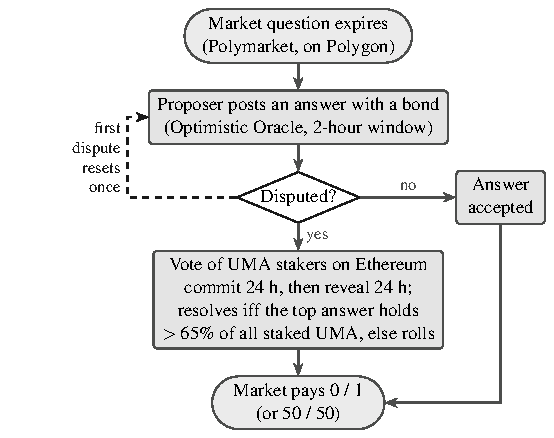
\includegraphics[width=0.98\columnwidth]{figures/fig_flow.pdf}
\caption{How a Polymarket question is settled. A proposer posts an answer with a bond to UMA's optimistic oracle on Polygon; an undisputed answer stands after two hours; a disputed one is reset once and, if disputed again, bridged to the Data Verification Mechanism (DVM) on Ethereum, where UMA stakers vote on the payout (the first dispute is voted on too, for its bonds only). The vote resolves only if the modal answer holds more than a threshold share of all staked tokens, otherwise it rolls to the next round and is deleted after four rolls. Numbered marks show what this paper measures: what the vote settles, the market's open interest (1); the margin by which the top answer's share of staked UMA clears the line (2); and the limit of any rule that turns the tally into a payout (3): the deployed rule pays in a step (solid), tally settlement in a ramp (dashed, Section~\ref{sec:mitigation}).}
\label{fig:flow}
\end{figure}

\section{Related work}
\label{sec:related}
We relate the paper to four lines of work.

\paragraph{Rational participants in deployed protocols}
\looseness=-1 Our method follows the work that models a deployed system's participants as rational, finds the equilibrium the designers did not intend, and repairs the mechanism: selfish mining under fee-driven rewards~\cite{carlsten2016,werlman2023}, consensus aware of maximal extractable value (MEV)~\cite{maddag2026}, symmetric and personal random reporting rewards~\cite{prrr2026}, side payments to proof-of-stake validators and the penalties on stake that counter them~\cite{bribing2024}, order-policy enforcement~\cite{diope2024}, payment channels~\cite{lightning2024} and fees under parallel execution~\cite{perils2026}. Relative to the closest, the side-payment analysis of~\cite{bribing2024}, the market being settled supplies the payment, so what a capture would collect is visible in the market, and voters who already favor the coalition's answer lower the stake it needs. Budish shows that the cost of protecting a blockchain must grow in proportion to what a manipulation would gain~\cite{budish2025}, and Budish, Lewis-Pye and Roughgarden ask when consensus can be costly to manipulate without a collapse of the token's value~\cite{blr2024}; Theorem~\ref{thm:limit} is the counterpart for a vote that settles markets, where the deterrent beside a 0.1\% penalty is the token's loss.

\paragraph{Schelling-point oracles and vote buying}
\looseness=-1 Schelling-point oracles pay voters for agreeing with the majority. Contingent payments for such votes are Buterin's $p+\epsilon$ construction~\cite{buterin2015} and Dal B\'{o}'s payments to committee members that are due only when a member's vote decides~\cite{dalbo2007} in token form, and UMA's roadmap names them as the open problem~\cite{umanextgen2025}; we add that no outside payer is needed when voters can hold the asset being settled and that the stake required is the threshold less the share that already votes for the coalition's answer. Freeman, Lahaie and Pennock pay each share of an arbitrated market the fraction of arbiters voting for it, observe that any binary settlement has a point where one arbiter moves a share by a dollar, and pay arbiters from trading fees for reports that agree with the others' (peer prediction)~\cite{freeman2017}. Tally settlement is their rule with a full dollar for any answer that wins a large enough majority; we add the bound for stake-weighted coalitions, the cost of that constraint and the limit (Theorems~\ref{thm:limit} and~\ref{thm:reach}), and Remark~\ref{rem:fees} prices their payments on a contested Polymarket market. Self-resolving markets pay their own final price~\cite{srinivasan2023}, and Appendix~\ref{app:tape} shows why that idea fails for contested votes. Deng, Tao and Wang show that once the share of voters working against the informed majority passes a threshold, no mechanism that treats voters alike can guarantee the majority's decision~\cite{dengtaowang2024}; Theorem~\ref{thm:tally} is the corresponding statement for deterministic stake-weighted tallies against voters who do not respond to the coalition, with the exact trade between the stake that captures and the stake that blocks, which quorum sizes govern in Byzantine agreement~\cite{malkhi2019}.

\paragraph{Oracle and market manipulation}
\looseness=-1 Price oracles in decentralized finance are manipulated by trading against the markets they read~\cite{eskandari2021,qin2021}; here the oracle is a vote and the market is what it settles. Proposition~\ref{prop:selffin} is the manipulation of a cash-settled contract through its settlement index~\cite{kumarseppi1992}, with a vote in place of the index. A manipulator who moves a prediction market's price can improve its accuracy~\cite{hanson2009}; a capturing coalition changes the payout and leaves the price alone. Section~\ref{sec:delta} draws on the catalogue of governance captures of~\cite{sokdao2024}; Kitzler et al.\ find a significant loss after 12 of 22 incidents involving decentralized autonomous organizations (DAOs), 13.5\% on average across those 12~\cite{kitzler2025}.

\paragraph{Other resolution designs}
\looseness=-1 Kleros decides by plurality of a stake-drawn jury and escalates through appeals~\cite{klerosdocs,kleros2021}, Augur by escalating bonds in its REP token that end in splitting the token by outcome~\cite{augur2019}, and Reality.eth by doubling bonds with a designated arbitrator~\cite{realitio}; a single Kleros round, like UMA's vote, resolves or rolls by its tally, while appeals and bonds leave that class of rules (Theorem~\ref{thm:tally} and Appendix~\ref{app:deployments}). UMA's votes have been measured by journalism, which reports that nine addresses dominate disputes and that most active voters hold Polymarket accounts~\cite{defiant2025,cryptonews2025,wsj2026,financemagnates2026,cryptobriefing2026}, and by studies of whether language models reproduce its resolutions~\cite{llmarbitration2026} and whether disputed markets price the event or its adjudication~\cite{wang2026}; voting power has been measured for DAOs~\cite{fritsch2024}. The census adds the margin of every vote, which votes decide a payout, the voters without whom a vote would have rolled, and the cost and the gain of a capture.

\section{Background}
\label{sec:background}

\subsection{Settlement on Polymarket}
\looseness=-1 Polymarket markets are Gnosis conditional tokens on Polygon: a binary market holds collateral in USDC and issues matching ``Yes'' and ``No'' shares, redeemable for one dollar each once a payout vector is reported~\cite{gnosisctf}. The adapter that reports it~\cite{polymarketadapter} asks UMA's Optimistic Oracle~\cite{umadvm2}. A proposer posts an answer, $1$ for Yes, $0$ for No, $0.5$ for an unresolvable question, or a reserved ``too early'' value, with a bond; a two-hour dispute window follows; anyone may dispute by matching the bond. Every dispute is sent through the Polygon bridge to the DVM, but the adapter re-asks the question on its first dispute under a new request, so the vote on that dispute decides only who keeps its bonds. The market is paid on the new request: on its proposal if undisputed, on the DVM's answer if disputed again. A ``too early'' answer from the DVM makes the adapter re-ask later. The current adapter also has an administrator, who can pause a question and report any payout for it an hour after flagging it.

\subsection{The DVM vote}
\looseness=-1 The DVM is a commit-reveal vote of UMA stakers held in rounds of 48 hours, 24 to commit and 24 to reveal. Revealed votes are public as they arrive. Each staker's weight is her staked balance at the start of the round. A request resolves at the end of the round to the modal answer $b^{*}$ if two conditions hold: the total stake that voted exceeds a fixed participation floor (5,000,000 UMA), and the modal answer's stake exceeds a fraction $\theta$ of \emph{all} staked tokens, not of the votes cast. Otherwise the request rolls to the next round, and after four rolls it is deleted. On resolution every staker who voted for another answer or did not vote loses $\lambda = 0.1\%$ of her stake, and the pooled penalties are divided among the voters of $b^{*}$ in proportion to stake. Nothing is paid or slashed in a round that rolls. The rule and its history are read from the contract source and from the parameter-change events it emitted (Table~\ref{tab:params}).

\begin{table}[t]
\centering
\caption{Parameters of the DVM vote, from the contract's parameter-change events.}
\label{tab:params}
\footnotesize
\renewcommand{\arraystretch}{0.9}
\setlength{\tabcolsep}{4pt}
\begin{tabular}{@{}llr@{}}
\toprule
Parameter & In force since & Value \\
\midrule
threshold $\theta$ & \deployDate & 50\% of staked \\
threshold $\theta$ & \spatChangeDate & 65\% of staked \\
participation floor & \deployDate & 5,000,000 UMA \\
penalty $\lambda$, wrong or absent & \deployDate & 0.1\% of stake \\
rolls before deletion & \deployDate & 4 \\
unstaking delay & \deployDate & 7 days \\
\bottomrule
\end{tabular}
\end{table}

\subsection{The vote of March 2025}
\label{sec:march-background}
\looseness=-1 Figure~\ref{fig:march} shows the reveal day of the request that decided the minerals-deal market's payout, read from the \texttt{VoteRevealed} events. Panel (a) accumulates the revealed stake for the two leading answers over the day; the three circles are the three wallets. Panel (b) is the market's own price of a Yes share, by the minute, from six hours before the last reveal to one hour after the round ended. The two panels show three facts the paper returns to: the vote's margin was smaller than any of the three wallets, the market did not believe the answer until it was forced to, and the hour between the last reveal and the end of the round was a window in which anyone reading the chain could buy a share worth a dollar for less than 35 cents.

\begin{figure*}[t]
\centering
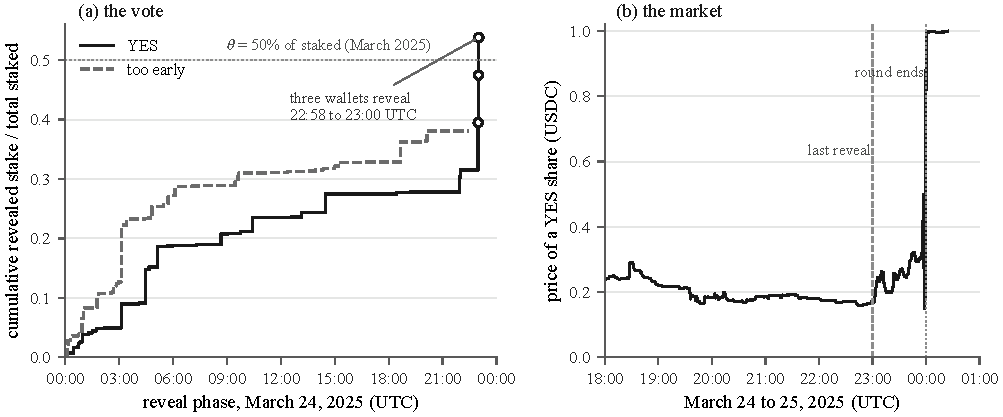
\includegraphics[width=0.96\textwidth]{figures/fig_march_timeline.pdf}
\caption{The March 2025 vote. (a) Cumulative revealed stake, as a share of all staked tokens, for ``Yes'' and ``too early'' during the 24-hour reveal phase of March 24, 2025 (UTC). The three circles are the three wallets that revealed between 22:58 and 23:00; the third took ``Yes'' past the 50\% line, which it cleared by \marchMargin{} UMA when the round ended. (b) The price of a ``Yes'' share on Polymarket by the minute. For nearly all of the hour after the last reveal the market sold Yes below 35 cents; the price reached 97 cents when the round ended.}
\label{fig:march}
\end{figure*}

\section{Model}
\label{sec:threat}
We describe who acts, write the vote in shares of the staked supply, and state the rules we compare and the guarantee we ask of them.

\paragraph{Participants}
A \emph{staker} holds UMA in the voting contract and votes once per request; her weight is her stake. A staker may also own shares of the market being settled; the Wall Street Journal reported in May 2026 that most active UMA voters could be linked to Polymarket accounts~\cite{wsj2026}, as summarized in~\cite{financemagnates2026}. The manipulator we study is a \emph{coalition}: it controls a share $\sigma$ of the staked supply, may split it across any number of wallets, may abstain, may hold any position $Q$ in the market being settled and in correlated markets, and sees every revealed vote as it arrives. It cannot change a commitment after the commit phase, cannot forge votes, and cannot read other voters' commitments. Polymarket's administrator can override the vote by flagging a question before its answer arrives, and on the managed oracle, which some markets have used since \managedSince{}, a resolver must settle each request before the market pays and can withhold that call (Sections~\ref{sec:background} and~\ref{sec:fork}); we study what the vote guarantees without either.

\paragraph{The rest of the electorate}
We describe the voters outside the coalition by two measured quantities: the \emph{honest bloc} $\hF$, the share of the staked supply that votes the coalition's answer $F$ for its own reasons, and the honest bloc $\hT$ that votes the opposing answer $T$. Both are read off the tallies of past votes. The guarantee of Theorem~\ref{thm:capture} and the cost--gain condition~(\ref{eq:budget}) allow any behavior of the rest of the stake; the other results fix every vote outside the coalition in advance, as the honest electorate defined below does.

\paragraph{Shares and tallies}
\label{sec:model}
A vote has a staked supply $S$, which we normalize to one when we write shares. The coalition holds a share $\sigma$ and votes $F$; an honest bloc $\hF$ votes $F$; an honest bloc $\hT$ votes $T$; the remaining share $m = 1 - \sigma - \hF - \hT$ votes as it likes or abstains. When all of it votes, we write $\varphi \in [0,1]$ for the fraction that votes $F$, and the tallies are
\[
x_F(\varphi) = \sigma + \hF + \varphi\,m, \qquad x_T(\varphi) = \hT + (1-\varphi)\,m .
\]
\looseness=-1 Under the deployed rule with threshold $\theta \ge 1/2$, $F$ resolves when $x_F > \theta$, $T$ resolves when $x_T > \theta$, and the request rolls otherwise; at most one of the two can exceed $\theta$. On resolution each losing or absent token pays $\lambda$, and the pool is shared by winning tokens in proportion to stake. These are the contract's rules; the only modeling choices are the normalization and the three blocs, and the blocs are measured from past tallies. We call the electorate \emph{honest} when the remaining share abstains; its \emph{participation} $\pi = \hF + \hT + \sigma$ is then the share of the staked supply that votes, and full participation is $\pi = 1$. In March 2025, for instance, the ``Yes'' votes outside the three wallets were \marchHF\% of the staked supply, so with a threshold of one half the wallets needed only \marchThetaMinusHF\% to carry Yes, and they held \marchAlpha\%. An honest electorate is one whose votes do not respond to the coalition. Voters who follow the coalition only lower what a capture needs, and voters with positions who change their votes count as part of the coalition (Section~\ref{sec:ramp-replay}).

\paragraph{Rules}
\looseness=-1 The deployed rule either resolves a vote or rolls it. We call any rule that maps the pair $(x, y)$ of shares voting $F$ and $T$ (abstention being $1 - x - y$) to $F$, $T$ or roll a \emph{resolve-or-roll rule}; the deployed rule and a single round of a Kleros jury are examples. A rule may instead turn the tally into a payout: it pays a Yes share $P(f)$ and a No share $1 - P(f)$, where $f$ is the share of the votes cast for Yes; \emph{proportional settlement}~\cite{freeman2017}, with $P(f) = f$, is one, and Section~\ref{sec:mitigation} proposes another. A rule of either kind is \emph{monotone} if more votes for an answer never hurt it ($F$ stays resolved when $x$ rises or $y$ falls; $P$ does not fall as $f$ rises) and \emph{neutral} if it treats the two answers alike (it is symmetric in them; $P(1 - f) = 1 - P(f)$). A resolve-or-roll rule is \emph{non-trivial} if a unanimous vote resolves, and it \emph{counts abstention as opposition} if an abstaining token weighs against an answer as a vote for the other answer does; the deployed rule, which measures each answer against all staked tokens, is one.

\paragraph{Goals and gains}
In these terms a \emph{manipulation} is a vote by the coalition that changes what a share pays: capture makes the vote resolve to $F$, and \emph{blocking} keeps the opposing answer $T$ from resolving, so that the question rolls. The coalition gains from capture through shares of $F$ bought below a dollar, through the penalty pool that resolution transfers to the winning side, and through anything settled by the same answer elsewhere. It pays through the carrying cost of its stake: purchase and price impact for a newcomer, the token's loss of value after a visible capture for an incumbent, and the penalty $\lambda$ if its side loses. We write $V$ for the market value of the staked supply and $\delta$ for the fraction of its value that a stake loses once a manipulation becomes visible, net of penalty-pool rewards. Payments to voters outside the protocol and bugs in the contracts are out of scope; the vote's own rules are the object of study.

\begin{definition}[Protection]
\label{def:protect}
A rule \emph{protects} the markets of a round at loss $\delta$ and participation $\pi$ if no coalition gains from manipulating them, whatever the honest electorate with that participation and whatever part of their open interest the coalition holds.
\end{definition}

\paragraph{What is public}
Stakes, votes, reveals, penalties and payouts are all on-chain. Our tallies use nothing else, and neither does the coalition.

\section{The limit of protection}
\label{sec:mitigation}
\looseness=-1 A rule that turns the tally into a payout can bound how far a coalition moves a payout, but it cannot make moving it costly; that cost is the stake's loss of value. The first result bounds the markets that any such rule can protect, and the rest of the section gives a rule that reaches the bound. Throughout, $\muparam \in [0, 1/2)$ and $\pi > 0$ is the participation of the honest electorate.

\begin{theorem}[The limit of protection]
\label{thm:limit}
For every monotone, neutral rule that pays a dollar to any answer with at least $1 - \muparam$ of the votes cast, some honest electorate and some coalition gain from manipulating a market whose open interest exceeds $\delta(1 - 2\muparam)\pi V$.
\end{theorem}
\looseness=-1 So no such rule protects a market whose open interest exceeds $\delta(1 - 2\muparam)\pi V$, three fifths of $\delta\pi V$ at $\muparam = 0.2$; protection is a worst-case guarantee. The reason is that a coalition's votes cost it the same loss of stake value under every rule, while the rule decides how far each unit of stake moves a payout. A rule that pays a dollar to any answer with $1 - \muparam$ of the votes must, by neutrality, pay nothing to one with $\muparam$, so its payout climbs a dollar across a band of width $1 - 2\muparam$. With $\muparam = 0.2$ and full participation, for example, honest blocs of a fifth on each side and a coalition holding the other three fifths move a market's payout by a dollar, at a cost of three fifths of $\delta V$. Per unit of stake the same electorate shows that no such rule keeps the worst-case movement of a payout below $1/(\pi(1 - 2\muparam))$. A rule whose payout jumps, as every rule that pays only zero or one does, is moved by the whole jump with an arbitrarily small stake. This is the observation of~\cite{freeman2017} for binary outcomes, in the language of stake, and the census finds contested votes close to the threshold (Section~\ref{sec:margins}). The proof of Theorem~\ref{thm:limit} in Appendix~\ref{app:proofs} covers all three claims.

\subsection{The rule}
\begin{definition}[Tally settlement]
\looseness=-1 Fix $\muparam \in [0, 1/2)$. A disputed question is settled on the tally of its first DVM round, whether or not the DVM resolves the request in that round. If ``too early'' alone leads the tally, or no vote is cast, the question is asked again, as today. Otherwise let $f$ be the share of the votes cast for Yes, a vote for one half counting half; a Yes share is paid
\[
\rho(f) = \min\Bigl\{1, \max\Bigl\{0, \frac{f - \muparam}{1 - 2\muparam}\Bigr\}\Bigr\}
\]
and a No share $1 - \rho(f)$. An undisputed question pays as the oracle says.
\end{definition}
\looseness=-1 With $\muparam = 0$ this is proportional settlement~\cite{freeman2017}. A vote for ``too early'' counts against Yes, since a Polymarket question resolves No unless Yes is established by its deadline: a minority saying that it is too early to settle lowers what Yes is paid, and a plurality has the question asked again. A vote won with $1-\muparam$ of the votes cast pays exactly as today; below that, the payout follows the tally. Polymarket already pays some questions at one half, and the conditional-token contract already accepts fractional payout vectors; tally settlement makes that outcome continuous in the tally. With $\muparam = 0.2$, the ``Yes'' of March 2025, which held \rampMarchVotesPct\% of the votes cast, would have been paid \rampMarchWithTwenty{} a share (Figure~\ref{fig:rule} in Appendix~\ref{app:ramp}). Without the three wallets ``too early'' would have led the round with \marchTooEarlyWithoutPct\% of the votes, and the question would have been asked again. The rule reads only the votes. Appendix~\ref{app:tape} explains why the obvious alternative, paying a contested vote at the market's own pre-dispute price, is not safe: a coalition that can force such a fallback buys the reference price back at no cost at settlement (Proposition~\ref{prop:selffin}).

\subsection{What the rule guarantees}
\label{sec:guarantee}
The second result says that tally settlement reaches the bound of Theorem~\ref{thm:limit} for every round.

\begin{theorem}[Tally settlement reaches the limit]
\label{thm:reach}
Under tally settlement, no coalition gains from manipulating the markets that one round settles when their open interest totals at most $\delta(1 - 2\muparam)\pi V$, with $\pi$ the smallest participation among them.
\end{theorem}
\looseness=-1 The proof rests on a range. Whatever a coalition does short of having the question asked again, its answer $F$ is paid between $\rho(\hF/\pi)$ and $\rho((\hF + \sigma)/\pi)$, so the coalition moves each share's payout by at most $\sigma/(\pi(1 - 2\muparam))$, whether or not the DVM resolves; its stake loses $\delta\sigma V$ once, however many markets the round settles. Proportional settlement moves a payout by $1/\pi$ per unit of stake and tally settlement by $1/(\pi(1-2\muparam))$, the least that any rule of Theorem~\ref{thm:limit} allows, so at $\muparam = 0.2$ and full participation a tenth of the stake moves a payout by at most \rampShiftTenPctTwenty{} cents. The bound is tight for a coalition that holds the whole other side. With $\muparam = 0$, proportional settlement protects up to $\delta\pi V$, and no rule that turns the tally into a payout protects more. From the range, a coalition can have $F$ paid a dollar if and only if $\hF + \sigma \ge (1 - \muparam)\pi$, at full participation $\sigma \ge 1 - \muparam - \hF$.

\looseness=-1 The rule keeps one delay. A coalition that wants the question asked again does best to vote ``too early'' with its whole stake, since a vote anywhere else lowers that answer's tally or raises a rival's; it then leads alone, and the question is asked again, exactly when $\sigma > \max\{\hF, \hT\}$. At full participation, where $\hT = 1 - \sigma - \hF$, that is $\sigma > \max\{\hF, (1 - \hF)/2\}$: with $\hF = 0.1$ it takes 45\% of the stake, where 25\% rolls the deployed vote at $\theta = 0.65$ (Section~\ref{sec:tally}). The proof of Theorem~\ref{thm:reach} is in Appendix~\ref{app:proofs}; the range and the delay were also checked by exact enumeration of every coalition split and every honest abstention on a grid.

\paragraph{Voters with positions, and disputes}
\looseness=-1 The coalition in Theorem~\ref{thm:reach} is any set of voters, so voters who hold positions move a payout together by at most their combined stake divided by $\pi(1 - 2\muparam)$; under the deployed rule they move nothing unless the vote turns on one of them, and then a dollar. A dispute changes what a share pays only if the side it favors ends with more than $\muparam$ of the votes cast, so disputing a clear outcome gains nothing, and a disputer with stake gains at most the bound above.

\section{Capture and blocking}
\label{sec:analysis}
\looseness=-1 Theorem~\ref{thm:limit} concerns rules that turn the tally into a payout. The deployed rule instead resolves a vote or rolls it and pays nothing or a dollar, so its payout jumps at the threshold. We derive the stake that capture and blocking need under it and under every resolve-or-roll rule, and turn the first into the budget of a capture.

\subsection{Two mechanical facts}
\label{sec:facts}
\looseness=-1 Two facts follow directly from the contract's rules; the \artifactlink{artifact} writes out both. First, blocking is free: a coalition holding at least $1-\theta$ of the staked supply that abstains keeps every answer from resolving, the request rolls each round and is deleted after four rolls, and the coalition is never charged a penalty, because penalties are computed only for resolved requests. Under the current parameters $1-\theta = 35\%$, and the four largest stakers hold \topFourPct\%. Second, the penalty pays the winner: if $b^{*}$ resolves with winning stake $v^{*}$, each winning token receives $\lambda\,(S - v^{*})/v^{*}$, and a coalition holding $\sigma S$ inside the winning side receives the share $\sigma S / v^{*}$ of the pool $\lambda (S - v^{*})$. In March 2025 the pool was \marchPool{} UMA and the three wallets' share \marchWhaleGain{} UMA. The transfer is small, and it runs from the voters who resisted the capture to those who made it. Appendix~\ref{app:proofs} adds a third fact.

\subsection{The capture threshold}
The next result gives the stake that makes capture certain.

\begin{theorem}[Capture]
\label{thm:capture}
\looseness=-1 If $\sigma > \theta - \hF$, then $F$ resolves in the current round whatever the remaining stake does. If $\hT \ge 1 - \theta$, then $F$ cannot resolve for any $\sigma \le 1 - \hT$.
\end{theorem}
\looseness=-1 Between the two regions the outcome depends on the rest of the stake, and both everyone voting $F$ and everyone voting $T$ can be equilibria, profiles from which no remaining voter gains by changing its vote (Proposition~\ref{prop:equilibria} in Appendix~\ref{app:proofs}). The honest bloc for the coalition's answer counts for it: every point of $\hF$ lowers the stake capture requires by a point. In March 2025 the honest bloc for Yes cut the requirement from one half to \marchThetaMinusHF\% of the supply, and the three wallets held \marchAlpha\%. By construction, their excess over the requirement is the \marchMarginPct\% by which the vote was won; what the theorem adds is the effect of the honest bloc, a guaranteed win for less than a fifth of the supply. Reading these ``Yes'' votes as followers of the three wallets only lowers the requirement further. Below the guarantee the remaining stake need not follow the three wallets. The global-games argument, which selects one equilibrium of a coordination game when players see the state with small noise~\cite{carlsson1993}, does not apply here, because the state of the world only moves which outcomes are feasible, and a numerical check of the vote with noisy signals in the \artifactlink{artifact} finds a continuum of equilibria below the guarantee. The cost side of the budget~(\ref{eq:budget}) starts from the guarantee. The proof is in Appendix~\ref{app:proofs}.

\subsection{What a threshold can and cannot do}
\label{sec:tally}
\looseness=-1 A higher threshold makes capture harder and blocking easier; the next result says by how much, for every resolve-or-roll rule. For a monotone, neutral, non-trivial resolve-or-roll rule let $\theta_f$ be the infimum of the $x$ at which $F$ resolves when everyone votes. Against an honest electorate, a bloc $\hF$ voting $F$ and everyone outside the coalition otherwise voting $T$, let $\sigcap(\hF)$ and $\sigblk(\hF)$ be the infima of the coalitions that make $F$ resolve and that keep $T$ from resolving.

\begin{theorem}[Resolve-or-roll rules]
\label{thm:tally}
For every monotone, neutral, non-trivial resolve-or-roll rule and every $\hF \le 1 - \theta_f$, $\sigcap(\hF) = \theta_f - \hF$ and $\sigblk(\hF) = 1 - \theta_f - \hF$, so that $\sigcap(\hF) + \sigblk(\hF) = 1 - 2\hF$ for every rule in the class.
\end{theorem}
\looseness=-1 This is the identity promised in the introduction; for larger $\hF$ the honest vote alone keeps $T$ from resolving. Every point that a rule adds to the stake needed to capture is taken from the stake needed to block, whatever the rule; the only thing a designer chooses is $\theta_f$, which fixes where the band of splits that resolve nothing sits, a band of width $2\theta_f - 1$ at full participation. The proof also shows how a coalition blocks best: voting $F$ blocks whenever any split of its stake does, and under a rule that counts abstention as opposition so does abstaining. Quorum sizes trade safety against liveness in Byzantine agreement in the same way~\cite{malkhi2019}. There a faulty node can vote for two values, so a larger quorum buys two units of safety for each unit of liveness it gives up; a staked token votes once, and the trade is one for one. Counting the threshold against votes cast instead of staked tokens leaves both formulas unchanged. It decides only whether a blocker may abstain or has to vote for the losing side, and because some honest voters abstain, it moves each requirement in staked supply by a point or two (at 96\% participation, \stakedTriggerBlockPct\% against \votesTriggerBlockPct\% for blocking with $\hF = 0$). The proof (Appendix~\ref{app:proofs}) is three monotonicity arguments; the appendix also records the variant in which the rest of the electorate may vote the blocker's own answer, which is where the denominator does matter and which honest voters do not produce. With more than two answers, honest votes for any answer other than the majority's count toward $\hF$ when blocking.

\looseness=-1 For the deployed rule, which resolves an answer only above $\theta$, the same electorate gives a window. A coalition of share $\sigma$ makes $F$ resolve whenever $\sigma > \theta - \hF$ and keeps $T$ from resolving whenever $\sigma \ge 1 - \theta - \hF$, so it can do neither exactly when $\theta \in [\sigma + \hF,\, 1 - \sigma - \hF)$, an interval that is non-empty if and only if $\sigma + \hF < 1/2$; the proof, for every $\hF \le \theta$, is in the \artifactlink{artifact}. The penalty, the participation floor and the rewards do not appear, and the honest bloc for the coalition's answer helps it on both sides. Today's four largest stakers hold $\sigma = \topFourShareExact\%$: no threshold protects a question from them once the honest bloc for their answer reaches \windowEmptyAtTopFour\%, and at $\theta = 0.65$ they capture a March-like question (requirement \captureReqSixtyFiveMarch\%) outright. The single largest staker (\topOnePct\%) cannot capture at 65\% unless the honest bloc for its answer exceeds \topOneCaptureNeedsHF\%, but it blocks any question on which more than \topOneBlockNeedsHF\% of the supply votes against the majority answer. In the census (Section~\ref{sec:census}), \nEraBContestedBlockableByTopOne{} of the \nPayoutContestedEraB{} contested payout votes since the change, and \nEraBBlockableByTopOne{} of all \nPayoutVotesEraB{} payout votes, had a winner below 65\% plus \topOnePct\% of the supply: a single stake the size of today's largest, voting the other way, would have rolled each of them. The 65\% change made capture harder and blocking easier by the same fifteen points.

\subsection{What the roadmap does not fix}
\looseness=-1 UMA's published plan for the next oracle generation names three directions: dynamic bonds that scale with a market's size, resolution by several tokens, and detection of vote buying through an external restaking layer~\cite{umanextgen2025}. Bonds live at the proposal stage and do not enter the vote; a second token changes $S$ and not $\theta_f - \hF$; and detection of vote buying presumes a payment to detect, whereas the market being settled itself pays whoever votes the right way in shares, indistinguishable from trading. All three stay inside the class of Theorem~\ref{thm:tally}.

\subsection{The budget of a capture}
\label{sec:identity}
\looseness=-1 The designers' argument is that their mechanism will ``ensure that the cost of corrupting the DVM will exceed the potential profit''~\cite{umaecon}. Theorem~\ref{thm:capture} and the second fact of Section~\ref{sec:facts} give the terms. Let $C(\sigma)$ be the cost of carrying a share $\sigma$ of the supply through one vote (two days of voting and seven days of unstaking): price impact plus the token's subsequent loss of value for a buyer, the loss of value alone for an incumbent. Let $\bar p$ be the coalition's average purchase price of claims paying a dollar on $F$, here or elsewhere, and $Q_{\max}$ the number it can buy at that price; its gains are these claims and the pool. In the limit $\sigma \downarrow \theta - \hF$ of the coalitions that capture for sure, which exist when $\hF \le \theta$ and $\hT < 1 - \theta$, cost exceeds the largest gain if and only if
\begin{equation}
\label{eq:budget}
C(\theta - \hF) \;>\; (1 - \bar p)\,Q_{\max} \;+\; \frac{(\theta - \hF)(1-\theta)}{\theta}\,\lambda V ,
\end{equation}
with $C$ continuous. We call (\ref{eq:budget}) the budget of a capture. Up to equality, it is thus necessary for safety against guaranteed capture, and it is sufficient when $C'(\sigma) \ge \lambda V(1-\theta)/\theta$ for $\sigma \ge \theta - \hF$, as when every staked token loses a common fraction of at least $\lambda(1-\theta)/\theta$ of its value (Appendix~\ref{app:proofs}). Three things differ from the argument as usually stated. The cost side carries $\theta - \hF$, not one half; the profit side grows with how unlikely the coalition's answer is, since $1 - \bar p$ is largest when that answer is cheapest; and the penalty appears on the profit side. In March 2025 the right-hand side was bounded by the \$\marchOIM{} million of open interest at the end of the round plus \marchWhaleGain{} UMA of penalties, and the left-hand side was whatever a visible capture cost the holders of \$\marchWhaleUsdM{} million of stake in the token's value. Under tally settlement the budget no longer involves the margin, the honest bloc or the size of the coalition, only the open interest a round settles against the value of the stake that votes (Theorem~\ref{thm:reach}).

\section{A census of the vote}
\label{sec:census}
We measure how close each vote was and who decided it.

\subsection{Data and method}
\label{sec:data}
\paragraph{Votes} We pulled every event of the voting contract (\texttt{VotingV2}, deployed \deployDate) from public archive endpoints up to \censusEnd: request additions, rolls, deletions, resolutions, every revealed vote with its stake, every stake change, delegation and parameter change. Resolutions are tallied from their \texttt{VoteRevealed} events in the resolving round, each request identified by its identifier, time and question text together, since requests that settle markets of one event share the first two; the staked supply of that round is read from the contract's frozen round record, which is the denominator the contract itself uses. For the two March 2025 requests we additionally decoded the penalty events the contract emitted and reproduced each voter's to the wei with a Python port of the contract's arithmetic (Appendix~\ref{app:port}).

\paragraph{Questions} Requests bridged after mid-2023 carry only a hash of the question and a Polygon block number. The question text, stamped by the oracle on Polygon, is in the event its bridge contract emitted at that block, and its Keccak-256 hash equals the one carried; every contested request matched.

\paragraph{Payout votes} A Polymarket question's first DVM request comes from its first dispute, after which the adapter has re-asked the question, so that vote decides only the bonds; later requests of the question decide the payout. The rule agrees with the chain for all \nRoleChecked{} contested requests matched to a market: only a first dispute's transaction re-asks the question. Of the \nPmQuestionsVoted{} Polymarket questions that reached the DVM, \nPmQuestionsOneVote{} reached it only once, for the bonds of their first dispute. The other \nNonPm{} votes are \nNonPmGov{} on UMA's governance, \nNonPmAcross{} disputes of Across bridge bundles (a disputed bundle is deleted, so the vote moves only the bond), \nNonPmYesNo{} questions asked on Ethereum and \nNonPmAssert{} assertions to UMA's Optimistic Oracle V3.

\paragraph{Markets} We match a question to its market without searching by title. Polymarket's adapter registers a question under the Keccak hash of the text it sent to the oracle, and the conditional-token contract identifies the market by the hash of the adapter's address, that question identifier and the number of outcomes, two. The oracle appends the adapter's address to the text before forwarding it, so the text in the voting contract yields both. We accept a derived market identifier only if the conditional-token contract on Polygon reports two outcome slots for it. For \nDerivedApiListed{} of the \nEconDerived{} contested requests matched this way, Polymarket's market API lists the market and returns the same question identifier; it lists none of the other \nDerivedApiMissing{}, whose markets exist on-chain. The adapter above is Polymarket's standard adapter. Neg-risk markets come in groups on mutually exclusive outcomes, between which positions can be converted; they are prepared by a different contract under a different question identifier, and we match those by exact title.

\paragraph{Open interest} A market's open interest at a block is the sum of its \texttt{PositionSplit} amounts minus the sum of its \texttt{PositionsMerge} amounts up to that block, from the conditional-token contract on Polygon; it is the number of complete Yes-and-No sets outstanding, each backed by one dollar. We take the last Polygon block whose timestamp is at most the end of the resolving round.

\paragraph{Prices} Token prices are Coinbase's public daily closes in UTC, so a close is the price at midnight UTC, when a voting round ends. Market prices are the market API's price history, by the hour for pre-dispute averages and by the minute around each vote's reveals. Every number in the paper is generated by one script from these sources.

\subsection{Participation and concentration}
Across the \nEraB{} votes since the 65\% change, the median request drew \votersMedEraB{} voters holding \partMedEraB{} of the staked supply; absence is slashed, so almost all of the stake votes. The supply is concentrated. In \censusEnd{} the largest staker held \topOnePct\% of \stakeNow{} staked UMA, the four largest \topFourPct\%, the ten largest \topTenPct\%. No single address has ever held 35\% of the supply (the maximum was \maxSingleEver\%); the smallest group of top stakers whose combined holdings reach 35\% has \kStall{} members, and reaching 65\% takes \kSixtyFive. The largest staker today is one of the three March 2025 wallets.

\subsection{Margins}
\label{sec:margins}
\looseness=-1 Figure~\ref{fig:winner} shows, for every resolved vote, the share of the staked supply held by the winning answer, separately for the two eras. Most votes are near-unanimous: the median winner held \winMedEraA{} of the supply before the change and \winMedEraB{} after. The lower tails are where the oracle is decided. Before the change \nEraAUnderSixtyFive{} of \nEraA{} votes had a winner below 65\%, every one of which would roll under the current rule; the minimum was \winMinEraA, the March vote. After the change the minimum is \winMinEraB, \nEraBWithinTwo{} votes sit within two points of the threshold, and \nEraBWithinTen{} within ten.

\begin{figure}[t]
\centering
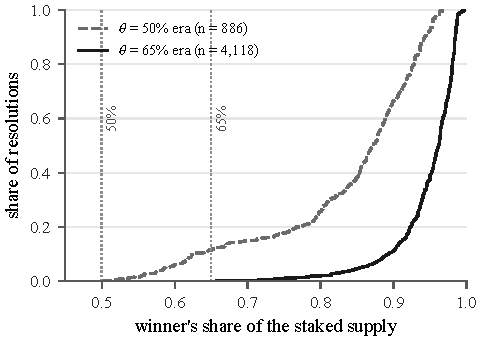
\includegraphics[width=0.98\columnwidth]{figures/fig_winner_share.pdf}
\caption{Winner's share of the staked supply at resolution, cumulative distribution over all resolved requests, before and after the threshold change of \spatChangeDate. The dotted lines are the two thresholds.}
\label{fig:winner}
\end{figure}

Of the \nContested{} contested votes, \nContestedPm{} were on Polymarket questions and \nPayoutContested{} of those decided a payout; the rest of this section counts these contested payout votes. The losing answers held a median \payMinorityMedian{} of the votes. The winner's margin above the threshold is \paySlackPTen{} of the supply at the tenth percentile and \paySlackMedian{} at the median, while the winner's largest single supporter holds \payTopSupporterMedian{} of the supply at the median and up to \payTopSupporterMax. Single-voter pivotality follows from these two distributions. In \nPayoutPivotal{} of the votes the winner falls below the threshold without its largest supporter, \nPayoutPivotalEraA{} before the change and \nPayoutPivotalEraB{} after; across all \nContested{} contested votes the count is \nPivotal. In all \nPayoutContestedEraB{} since the change, removing three supporters or fewer suffices. In \nPayoutPivotalYesNo{} of the \nPayoutPivotal{} the winner was Yes or No; in the other \nPayoutPivotalTooEarly{} it was ``too early'', and the largest supporter chose between two delays, asking the question again at once or voting on it again after a roll. Removing a supporter rolls a vote; carrying another answer is harder, and in only \nPayoutPivotalFlipWord{} of the \nPayoutPivotal{} would the largest supporter's stake, voting for the runner-up, have made it win. The ``too early'' answer wins \nPayoutTooEarlyWins{} of the \nPayoutContested, and in those the dispute was over whether the question could be settled yet.

\subsection{The March 2025 vote in detail}
\label{sec:march}
The market was the subject of two requests in this round. The first came from the first dispute, after which the adapter had already re-asked the question; ``Yes'' won its vote by \marchFirstMarginPct\% of the stake with the same three wallets pivotal, and that vote decided only the dispute's bonds. The second request decided the payout, and Table~\ref{tab:march} in Appendix~\ref{app:port} collects its reconstruction. The threshold was half the staked supply, \marchStake{}$/2$ UMA. ``Yes'' cleared it by \marchMargin{} UMA. Without the three wallets, ``Yes'' would have held \marchYesMinusWhalePct\% of the supply and ``too early'' \marchTooEarlyPct\%; neither resolves, the request rolls. We checked this against the deployed code. On a fork of Ethereum mainnet taken one block before the first of the three reveals (block \forkReplayBlock), we replayed every later reveal of the request with its original sender, calldata and timestamp: the contract resolves the request when the round ends, and it rolls the request if the reveal of any one of the three wallets is left out, even that of the smallest, which held \marchWalletCPct\% of the supply. Each wallet alone was pivotal. The three wallets' \marchWhale{} UMA was \marchWhaleShareOfWinners\% of the winning side, and the penalty pool of \marchPool{} UMA, drawn from the \marchTooEarly{} UMA that voted ``too early'' and the \marchAbstain{} UMA that did not vote, paid them \marchWhaleGain{} UMA. At the day's price of \$\umaPriceMarch{} per UMA the staked supply was worth \$\marchStakeUsdM{} million and the three wallets' stake \$\marchWhaleUsdM{} million.

What could capture have earned? When the round ended, \marchOI{} sets of this market were outstanding, read from the conditional-token contract's split and merge events on Polygon; the market's \$\marchVolumeM{} million of volume was turnover. In the following week \marchRedeemers{} wallets redeemed \$\marchRedeemed{} of Yes shares, the five largest \marchTopFiveSharePct\% of the total; the redemptions exceed the sets outstanding at the vote because new sets were created after it. Between the request reaching the vote and the last reveal, \marchDisputeBuyWallets{} wallets bought \marchDisputeBuyShares{} Yes shares for \$\marchDisputeBuyCost{}. In the hour between the last reveal and the end of the round, when the outcome was readable on-chain, \marchPostRevealWallets{} wallets bought \marchPostRevealShares{} for \$\marchPostRevealCost{}, at \marchPostRevealLowCents{} to \marchPostRevealHighCents{} cents for fifty minutes and up to \marchPostRevealMaxCents{} cents in the last ten.

Once the winner's revealed stake passes the threshold, no other answer can reach it, so in every vote the outcome is fixed and public before the round ends: across the \leakMarkets{} contested Yes-or-No markets with minute prices, a median of \leakLeadMedianH{} hours before. Usually the market had priced the answer already, above 90 cents in \leakHigh{} of them when the deciding reveal landed. The exception is March 2025, where Yes stood at \leakMarchCents{} cents when the outcome was fixed and the price caught up only as the round ended. A coalition need not hold a position before the vote: when the market is slow, it can buy one after its own reveal.

Who held the stake? The three wallets first staked in \whaleFirstStakeDate, within \whaleFirstStakeHours{} hours of each other and a week after the contract went live, and none of them staked tokens of its own again before the vote. The only additions were voting rewards, which two of the wallets re-staked \whaleRestakesA{} and \whaleRestakesB{} times, \whaleRestakesPaired{} times within two minutes of each other. The joint schedule, the common start and the reveal times are why we treat the three as one actor; we have no funding-chain evidence for it. On that reading the capture was made with stake held for two years. Two conclusions follow. A single market of this size cannot pay for a seven-million-dollar stake bought for the purpose, so the economics of capture are those of an incumbent, whose cost is the token's loss of value rather than a purchase (Section~\ref{sec:budget} measures that loss); and the mechanism's own penalty pointed the wrong way, small as it was.

\subsection{What the 65\% change did}
\label{sec:change}
\looseness=-1 The change did what its proposal said it would: weak majorities now roll and give voters more time~\cite{umaspat2025}. The proposal estimated that 6 of 291 requests in 2025 would have rolled under the new threshold; over the same year up to the change, our census counts \nTwentyTwentyFiveUnderSixtyFive{} of \nTwentyTwentyFiveBeforeChange{} votes whose winner held 65\% of the supply or less, consistent with that estimate. What the change did not do is make contested votes safer. Repeated rolls rose: before the change \nRolledEraA{} requests rolled and \nRepeatRollsEraA{} rolled twice; after it \nRolledEraB{} rolled, \nRepeatRollsEraB{} rolled two or more times, and one request rolled four times and was deleted (its question text was a hash the voters could not read, so nobody manipulated it; a blocked question ends this way, leaving the oracle). Single-voter pivotality continued, \nPivotalEraB{} cases, \nPayoutPivotalEraB{} of them on votes that decided a payout, with winners just above the new line and largest supporters of ten percent of the supply. Theorem~\ref{thm:tally} explains why: the threshold moves the stake needed to capture and the stake needed to block in opposite directions by the same amount.

\section{What a capture could collect}
\label{sec:collect}
We measure the budget of a capture on every contested Polymarket vote, and when its prize was minted.

\subsection{The budget, measured}
\label{sec:budget}
\looseness=-1 We read both sides of (\ref{eq:budget}) from the chain for every contested Polymarket question. The profit side is bounded by the market's open interest when the vote closed. Of the \nEconContested{} contested Polymarket votes, \nEconMatched{} match their market (Section~\ref{sec:data}), \nEconDerived{} through the market identifier derived from the question text and the rest, neg-risk markets, by exact title. Of these, \nEconPayoutRequests{} decided a payout and form \nEconMarkets{} distinct pairs of market and round; the other \nEconBondOnlyRequests{} were first disputes. The cost side is the \emph{capture stake}, the stake that would have carried $F$, the side the vote did not choose (the side with more votes when the vote said ``too early''). By Theorem~\ref{thm:capture} an incumbent needs $\theta - \hF$ of the supply, with $\hF$ the share $F$ actually received, and we value that stake at the token's closing price on the day the vote closed. The ratio $r$ of open interest to that value bounds the fraction of the capture stake's value that a capture can destroy and still pay.

\looseness=-1 Figure~\ref{fig:budget}(a) shows both sides. The median market held \$\econOIMedian{} of open interest, the median capture stake was worth \$\econVMedianM{} million, and the median $r$ was \econDeltaMedianPct\%. In \econDeltaGeTenth{} of these votes the open interest exceeded a tenth of the capture stake's value, and in \econDeltaGeOne{} it exceeded all of it: there, even the token's total loss would not have ruled out a profitable capture.

\looseness=-1 Before the 65\% change \econDeltaGeTenthEraA{} of \econMarketsEraA{} votes had $r \ge 0.1$; since, \econDeltaGeTenthEraB{} of \econMarketsEraB{}, so the tail has grown. The higher threshold raised the stake a capture needs by fifteen points, but over the same period the token fell from \$\umaPriceMarch{} at the March vote to \$\umaPriceNow{} at the end of the census, taking the value of the staked supply from \$\marchStakeUsdM{} million to \$\stakeNowUsdM{} million, while the largest markets grew. When the vote on ``Israel x Hezbollah ceasefire by April 18, 2026?'' closed, its market held \$\econTopOIM{} million of open interest, \econTopOverStake{} times the value of the staked supply; the stake its capture needed was worth \$\econTopVM{} million, and the staked supply \$\econTopStakeValueM{} million. Table~\ref{tab:budget} lists the ten largest ratios.

\looseness=-1 Who could have collected? The \econDeltaGeOne{} votes with $r \ge 1$ each needed at least \econMinSigmaDeltaOnePct\% of the supply, because almost nobody had voted the other side; the ten largest stakers today hold \topTenPct\% together. A coalition the size of today's four largest stakers (\topFourPct\%) could have carried the other side in \econCapTopFour{} votes, with ratios of at most \econMaxDeltaTopFour, and the largest single stake (\topOnePct\%) in none. The budget fails where the designers' argument looks, at coalitions of half the stake or more valued at market prices, and not for today's largest stakers acting alone. What a single stake decides is whether a vote resolves (Section~\ref{sec:margins}).

\begin{figure*}[t]
\centering
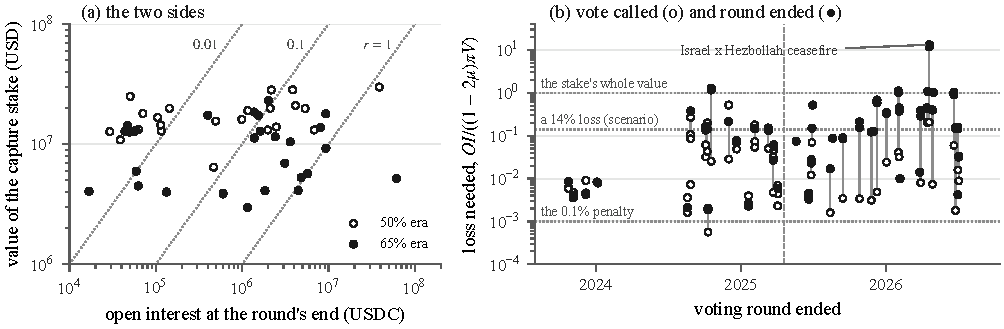
\includegraphics[width=0.96\textwidth]{figures/fig_budget.pdf}
\caption{The budget of the contested votes that decided a payout. (a) Open interest when the vote closed against the value of the capture stake, the share $\theta - \hF$ that would have carried the other side; dotted lines mark $r$ of 1, 0.1 and 0.01. (b) Per round, the loss of stake value that tally settlement with $\muparam = 0.2$ (Section~\ref{sec:mitigation}) needs at the participation $\pi$ of the round's first vote, $\mathrm{OI}/((1-2\muparam)\pi V)$ with OI the open interest (Theorem~\ref{thm:limit}), with the open interest when each standard-adapter market's vote was called (hollow) and when the round ended (filled); the dashed line is the threshold change.}
\label{fig:budget}
\end{figure*}

\begin{table*}[t]
\centering
\caption{The ten contested payout votes with the largest ratio $r$ of open interest (OI) when the vote closed to the market value of the capture stake; amounts in millions of dollars.}
\label{tab:budget}
\footnotesize
\setlength{\tabcolsep}{4pt}
\begin{tabular}{@{}llccccrrr@{}}
\toprule
Question & Closed & $\theta$ & Vote & $F$ & $\hF$ & OI & Stake & $r$ \\
\midrule
Israel x Hezbollah ceasefire by April 18, 2026? & 2026-04 & 65\% & Yes & No & 1.4\% & 61.4 & 5.2 & 11.86 \\
Will Trump launch a coin before the election? & 2024-10 & 50\% & Yes & No & 0.0\% & 38.6 & 29.9 & 1.29 \\
Will ``Donk'' be said during the PGL Bucharest 2026 Grand Final? & 2026-04 & 65\% & No & Yes & 14.5\% & 4.4 & 4.1 & 1.08 \\
Clavicular pregnancy in 2026? & 2026-04 & 65\% & Yes & No & 0.0\% & 5.7 & 5.7 & 1.01 \\
Tesla launches unsupervised full self driving (FSD) by June 30? & 2026-02 & 65\% & Yes & No & 0.2\% & 9.3 & 9.3 & 1.01 \\
Will Trump agree to withdraw troops from the Iranian region by June 3\ldots{} & 2026-06 & 65\% & Yes & No & 0.0\% & 4.8 & 5.3 & 0.91 \\
Trump declassifies UFO files in 2025? & 2025-12 & 65\% & Yes & No & 0.0\% & 8.1 & 13.8 & 0.59 \\
Fordow nuclear facility destroyed before July? & 2025-06 & 65\% & Yes & No & 0.5\% & 9.3 & 17.9 & 0.52 \\
Israel x Hezbollah Ceasefire in 2024? & 2024-11 & 50\% & too early & Yes & 28.3\% & 6.8 & 13.1 & 0.52 \\
Will Trump talk to Vladimir Putin in January? & 2026-02 & 65\% & No & Yes & 16.9\% & 3.1 & 6.9 & 0.45 \\
\bottomrule

\end{tabular}
\end{table*}

\looseness=-1 Open interest overstates what a coalition can collect, since it must buy $F$ from holders willing to sell, so we also measure what it could have bought. A coalition that means to carry $F$ buys it while it is cheap and before its own reveal. Taking each market's actual trades from the request reaching the vote to the decisive reveal, we let the coalition take the place of the wallets that bought $F$ on net, at their own average prices, so that a share bought and resold inside the window counts once. If $F$ is then paid a dollar, the coalition collects \$\execMedian{} in the median market, \execOverOIMedianPct\% of the open interest, and up to \$\execMaxM{} million; this revenue exceeds a tenth of the capture stake's value in \execGeTenth{} votes and all of it in \execGeOne.

\looseness=-1 An incumbent should compare it with the whole stake it puts at risk: a coalition the size of today's four largest stakers could have collected at most \execTopFourMaxPct\% of its stake's value from any market it could have captured, and one the size of today's largest could have captured none. Open interest says where no loss of stake value could guarantee safety; the revenue from the trades that took place says where a capture would have paid; whether any capture did pay would need the coalition's identity and positions, which the chain does not reveal. Capturing a single contested market pays such a coalition only if a visible capture costs its token less than a few percent. Conversely, a buyer of stake pays more than the market value of the capture stake, since buying moves the price.

\looseness=-1 The cost side for an incumbent is the token's loss of value, and the March vote shows what that loss was. The three March 2025 wallets held stake worth \$\marchWhaleUsdM{} million. The market's trades would have let them collect \$\execMarch{} on Yes: \$\execMarchDispute{} before the reveals began, \$\execMarchReveal{} before their own reveals, and \$\execMarchAfter{} after them, when the outcome was fixed on-chain and the market still sold Yes cheaply. If the three were one actor, the capture paid if it cost the token less than \execMarchWhalePct\% of its value, less than one day's standard deviation of UMA's return relative to ETH (\econSdEthOne{} points), and the token showed no loss of that size (Appendix~\ref{app:delta}): its price could not have told anyone whether the capture paid.

\subsection{When the prize is minted}
\label{sec:prize}
\looseness=-1 Most of the open interest measured when a vote closes did not exist when the vote was called. A disputed question waits \prizeVoteHours{} hours at the median for its round to end while its market trades on, and each purchase of the expected answer near a dollar mints a set whose other half sells near a tenth of a cent. A budget of a capture checked when the question is disputed therefore weighs the stake against a prize that is still growing. For the \prizeN{} contested payout votes on the standard adapter we read the open interest at the block of the dispute that sent the payout vote's request to the DVM and at the end of its first round, on which tally settlement pays. It grew from \$\prizeEscM{} million to \$\prizeFirstM{} million, so \prizeAfterPct\% was minted after the vote was called; the twenty largest markets grew \prizeVoteGrowth-fold at the median, against \prizePreGrowth-fold over an equal span before the dispute. No market had $r \ge 1$ when its vote was called, and \prizeDeltaOneFirst{} did when the round ended. Halting a market's order book while its question is before the DVM stops this minting (Section~\ref{sec:deploy}): with the open interest at the dispute, the loss that tally settlement needs (Figure~\ref{fig:budget}(b)) would have stayed below the value of the staked supply for every market and below \deltaDetectablePct\% for all but \prizeReqDetEsc, though a coalition could still buy before disputing.

\looseness=-1 The ceasefire market shows it at full size: called with \$\cfOIEscM{} million of open interest, it held \$\cfOIDayM{} million a day later and \$\cfOIEndM{} million when the round ended, \cfGrowth{} times as much. Before the reveals, buyers paid \cfYesCents{} cents on average for \cfYesM{} million ``Yes'' shares, and \cfBuyers{} wallets bought \cfNoM{} million ``No'' shares on net, \cfTickPct\% of the volume at a tenth of a cent and the largest buyer about \cfLargestBuyerPct\% of it. At their prices, a coalition in the place of these buyers would have held \cfNoTotalM{} million shares for \$\cfCostTotal{} up to the decisive reveal (the market charged no fees), a claim to \$\cfNoTotalM{} million settled by its own votes. With \cfHNoPct\% of the stake voting ``No'' honestly, it needed \cfNeedPct\% (Theorem~\ref{thm:capture}), held by the round's \cfCoalitionK{} largest voters, the largest with \cfLargestVoterPct\%. Charged the value of the staked supply, \$\cfStakeM{} million, the capture pays up to \cfOverStake{} times its cost net of the purchase; half the shares at ten times the price would still pay \cfHalfTenX{} times, and the capture loses only for a coalition holding more than \cfOverAllUma{} of all UMA in existence, staked or not.

\section{The limit on UMA's markets}
\label{sec:uma}
We replay tally settlement on the oracle's history and apply the limit to its markets.

\subsection{What the rule would have paid}
\label{sec:ramp-replay}
\looseness=-1 Because the rule needs only tallies, we replay it over every Polymarket vote that decided a payout, on the first round of each (Table~\ref{tab:ramp} in Appendix~\ref{app:ramp}). Of the \rampYesNoBothPay{} Yes-or-No votes both rules pay, tally settlement with $\muparam = 0.2$ pays \rampCutTwenty{} less than in full (\rampCutPctTwenty\%), by a median of \rampHaircutTwenty{} cents, \rampCutEraBTwenty{} of them since the 65\% change; proportional settlement pays \rampCutZero{} less than in full, mostly by a fraction of a cent. Of the \rampContestedSidedN{} contested Yes-or-No votes, the winners would have been paid a full dollar in \rampWinnerFullTwenty{} and \rampWinnerPTenTwenty{} or more in nine of ten. At full participation a tenth of the supply moves any payout by at most \rampShiftTenPctTwenty{} cents, and a one-dollar capture of a March-like question needs \rampCaptureMarchTwenty\% of the supply. In the \rampPivotalN{} single-voter-pivotal Yes-or-No votes the largest supporter moves the winner's payout by a median of \rampPivotalMedianCentsTwenty{} cents and at most \rampPivotalMaxCentsTwenty, since the roll it could cause no longer moves the payout. The replay keeps the votes outside the replayed coalitions as cast; voters who know that the payout follows the tally may vote, abstain or dispute differently, and Theorems~\ref{thm:limit} and~\ref{thm:reach} cover abstention through $\pi$ and count voters with positions who change their votes as part of the coalition.

\looseness=-1 Coalitions the size of today's largest stakes show the trade the rule makes. In the \coalEraBN{} contested Yes-or-No payout votes since the change, a stake the size of today's largest (\topOnePct\%) that switches from the winner to the other side rolls \coalTopOneRoll{} of them under the deployed rule and flips none; under tally settlement it moves the winner's payout by a median of \coalTopOneMedianCents{} cents and at most \coalTopOneMaxCents. A coalition the size of the four largest rolls all \coalTopFourRoll{} and moves the payout by a median of \coalTopFourMedianCents{} cents and at most \coalTopFourMaxCents. The deployed rule lets such stakes delay; tally settlement lets them move money, in proportion to their size and never by the whole dollar. They can still delay by voting ``too early'' (Section~\ref{sec:guarantee}): moved to that answer, the largest stake would have had \coalTopOneAskAgain{} of the \coalEraBN{} questions asked again, and the four largest \coalTopFourAskAgain. The rule's price is this shortfall: a vote that is right but contested pays its winners less than a dollar, by an amount set by the share the losers held.

\subsection{How much loss each market needs}
\label{sec:cap}
\looseness=-1 Theorem~\ref{thm:limit} turns the budget of Section~\ref{sec:budget} into one number per market: the loss of stake value $\delta$ a market needs before any rule that pays supermajorities in full can protect it at the participation of its first round. In the \rampMarkets{} contested payout votes the participation of the first round ranged from \piFirstMinPct\% to \piFirstMaxPct\% of the staked supply, with a median of \piFirstMedPct\%. The only loss the oracle imposes is its penalty and the pool reward a manipulator forgoes, at most $\lambda/\theta$ of a voter's stake in all, and a coalition large enough to block avoids both (Remark~\ref{rem:penalty}, Appendix~\ref{app:proofs}). With $\delta = \lambda/\theta$ the limit is at most about \$\penaltyCapUsd{} at the end of the census, and the markets of all \rampMarkets{} contested payout votes held more. Beyond the penalty, $\delta$ is the token market's verdict on a manipulation, which Section~\ref{sec:delta} measures. With $\muparam = 0.2$, the median market is protected once $\delta$ exceeds \rampDeltaNeedMedianPct\%; \rampNeedTenth{} markets need more than a tenth, \rampNeedQuarter{} more than a quarter, and \rampNeedOne{} more than the value of the staked supply. The ceasefire market of Section~\ref{sec:budget} is beyond the worst-case guarantee of every rule that turns the tally into a payout, proportional settlement included, even with $\delta = 1$. Counted by round, as the limit requires, those needing more than a tenth rise from \rampNeedTenth{} to \roundNeedTenth, and those beyond the value of the staked supply remain \roundNeedOne.

\subsection{What a visible manipulation costs}
\label{sec:delta}
\looseness=-1 To measure $\delta$ we take the captures and attempted captures of on-chain votes in the catalogue of Feichtinger et al.~\cite{sokdao2024} that have a public date and a year of daily prices, and two later ones, Compound's treasury vote of July 2024~\cite{invezz2024} and UMA's of March 2025; Appendix~\ref{app:delta} gives the method and the \deltaEvents{} cases. Where a capture drained or diluted the protocol itself, the governance token lost a median \deltaDrainedMedianPct\% of its value against ETH in the week, significantly in \deltaDrainedSig{} of \deltaDrainedN. A capture of Polymarket's settlements takes nothing from UMA, and none of the \deltaCleanN{} captures and attempts that took nothing from their protocol had a significantly negative week; their median loss was \deltaCleanMedianLossPct\%, and the one-sided 95\% bound on their mean is \deltaBoundAllPct\%. The sample detects a mean loss of \deltaDetectablePct\% only four times in five, so \deltaDetectablePct\% serves below as a scenario for UMA. At that loss the markets of \deltaUnprotectedAtDetectable{} of the \rampMarkets{} contested payout votes lie beyond the rule's guarantee, and in \deltaBuyableBeyond{} of them the shares a coalition could have bought from the market's own trades exceed the limit by themselves. Conversions may inflate the open interest of the \negRiskMarkets{} votes on neg-risk markets; without them \deltaUnprotectedWoNegRisk{} of these \deltaUnprotectedAtDetectable{} remain beyond the limit, and all \rampNeedOne{} beyond $\delta = 1$.

\subsection{What follows for deployment}
\label{sec:deploy}
\looseness=-1 The first remedy works on the prize. Polymarket's operator matches orders off-chain and settles the matches on-chain~\cite{ctfexchange}, so halting a market's order book once its question goes to the DVM stops the purchases that mint new sets. Anyone can still split collateral into sets on the conditional-token contract, but a set returns exactly its cost under any payout, so it gains a coalition nothing unless the other half can be sold. The prize is then at most the open interest at the dispute, which the operator can weigh against the stake before the vote (Section~\ref{sec:prize}), at the price of \prizeVoteHours{} hours at the median without trading in a disputed market. A coalition's stake moves every question in a round, and anyone can bring a question to the vote by disputing its proposals (Section~\ref{sec:background}), so the open interest to weigh is the total that one round settles: choose the loss of stake value $\delta$ to rely on and cap that total at $\delta(1 - 2\muparam)\pi V$, or add stake; no rule that turns the tally into a payout protects more. Asking a question again when less than a share $\pi_0$ of the staked supply votes in its first round makes the cap hold with $\pi_0$; the DVM's own participation floor does not, since tally settlement pays whether or not the DVM resolves. Settle disputed questions by the tally, with $\muparam$ read off Table~\ref{tab:ramp}: among rules that pay a full dollar to any answer with at least $1 - \muparam$ of the votes cast it reaches the limit, and the threshold change of April 2025 then stops mattering for what a share pays. The rule needs one new input, the first round's tally by answer, and no market data. It applies as built to the standard adapter; Polymarket's neg-risk contract accepts only the payouts $[1,0]$ and $[0,1]$, so those markets need a contract change first.

\section{Replays on the deployed contracts}
\label{sec:fork}
We replay two votes on local forks of both chains to check that the deployed contracts do what the arithmetic says.

\looseness=-1 \paragraph{The capture} On local forks of both chains, the round's \cfCoalitionK{} largest voters on the ceasefire question vote ``No'', and every other vote of the round is replayed as cast. The live voting contract resolves ``No''. This market is on the managed oracle, as are \nManagedPayout{} of the \nPayoutContested{} contested payout votes. With the bridge's delivery and the resolver's call simulated, the deployed oracle, adapter and conditional-token contract pay ``No'', and the vote's \forkCfHolders{} largest ``No'' buyers redeem \forkCfHeldM{} million shares for \$\forkCfPaidM{} million. Unchanged, the same replay pays them nothing; under capture the coalition's stake rises by \forkCfStakeGain{} UMA over the round. The \$\forkCfPaidM{} million is \forkCfOverStake{} times the value of the staked supply. The replay checks the two facts that the counterfactual of Section~\ref{sec:prize} assumes: by the contract's own accounting the coalition's stake carries the round, and no contract check between the vote and the payout stops a captured answer. Two roles remain: the resolver, who can delay the payout by withholding its call but cannot change the answer, and the adapter's administrator, who can flag the question before the answer is delivered and settle it by hand an hour later (Section~\ref{sec:background}); the replay leaves the administrator out.

\looseness=-1 \paragraph{Blocking} The latest contested payout vote whose answer pays, ``Will Donald Trump publicly insult someone on June 21, 2026?'' (\$\forkBlkOIK{} thousand of open interest), is forked the same way. Its four largest voters, \forkBlkCoalitionPct\% of the stake, vote ``Yes''; ``No'' falls to \forkBlkNoPct\% and the question rolls. In constructed later rounds every voter votes as before; the contract rolls the question \forkBlkRolls{} times and deletes it in the fifth round, charging no one for it. On Polygon the adapter then cannot resolve, and the collateral stays locked until an administrator of the adapter flags the question and, an hour later, reports a payout of its choosing. A coalition that can block hands the settlement to the adapter's administrator.

\section{Prototype}
\label{sec:prototype}
\looseness=-1 Tally settlement needs the vote's tally on Polygon, where the adapter runs; the tallies live in the voting contract on Ethereum. The prototype (Solidity 0.8.24, Foundry~\cite{foundry}) has three parts. \emph{MarginReader} (Ethereum) takes a resolved request's identifier and index, checks one against the other, and stores the winner's share in basis points for the bridge. Read against the staked supply it runs on today's contract: on a mainnet fork it returns \forkMarginA{} and \forkMarginB{} basis points for the two March 2025 requests and rejects a wrong index. The version the rule needs reads Yes's share of the votes cast, a vote for one half counting half, or a flag to ask again when ``too early'' led the round; it needs one view, the round's tally by answer, which the deployed contract stores but does not expose, and on a mock with the March tallies it returns \marchYesVotesBps{} basis points. \emph{TallyAdapter} (Polygon) pays a question settled without a vote as the oracle says and a disputed one $\rho(f)$ to Yes and the rest to No; ten tests cover the March tallies (\rampMarchBps{} basis points to Yes), the full-payment threshold, the one-half and ask-again cases, and a fuzz test of the bound $\sigma/(1-2\muparam)$. Two tunnels carry the share to Polygon. A disputed question costs about \gasRegister{} gas on Ethereum once and at most \gasTallyRamp{} on Polygon once, and nothing recurs per trade; the \artifactlink{artifact} lists the gas of each call.

\section{Ethics, AI use and artifact}
\label{sec:discussion}
\paragraph{Ethics}
\looseness=-1 Every input to this paper is public: on-chain events, public APIs and published documentation. Addresses are pseudonymous and we do not attempt to identify their owners; the attribution of three wallets to one actor is stated as an inference. No transaction was sent to any live contract; the counterfactuals are computations, and the replays and the prototype ran on local forks and in unit tests. The weaknesses discussed follow from parameters the operator published and from a vote the operator and the press have already analyzed; the paper adds measurement and a design analysis. Before submission we reported the measurements, the analysis and the remedies to Polymarket through the private vulnerability-reporting channel of its adapter repository on \disclosurePolymarketDate{} and, since the remedies on the oracle's side are governance decisions, posted them on UMA's governance forum, where its parameters are proposed, on \disclosureUmaDate{}; we offered both the \artifactlink{artifact}.

\paragraph{AI disclosure}
\looseness=-1 Generative AI tools, including Codex and Claude, assisted with literature searches, coding assistance and prose polishing. The authors conceived the paper's core ideas, developed its methods, verified the correctness and originality of all content, including the references, and take full responsibility for it.

\paragraph{\artifactlink{Artifact}}
\looseness=-1 The \artifactlink{anonymized artifact} contains every script with the decoded per-request summaries, the exact-arithmetic checks, the slashing port, the replays on forks of both chains, both prototypes with their tests, and the proofs.

\section{Conclusion}
\looseness=-1 A stake-voted oracle protects a market only while it is worth less than what a visible manipulation would cost the stake that votes, and no rule that turns the tally into a payout changes that. On Polymarket's oracle these markets grow after their questions go to the vote. In April 2026 one market grew \cfGrowth-fold during its vote, to \econTopOverStake{} times the value of the staked supply, and on forks of both chains the deployed contracts paid a captured vote in full after the resolver's call. The oracle's own penalty protects a few thousand dollars, and nothing against a coalition that can block. The margin is a second weakness: it has been one voter wide on \nPayoutPivotalWord{} contested votes that decided a payout, and raising the threshold moved fifteen points of weakness from capture to blocking. Halting trading while a question is before the vote caps the prize at its size when the vote was called.

\bibliographystyle{IEEEtran}
\bibliography{refs}

\appendices
\renewcommand{\arraystretch}{0.85}

\section{Proofs}
\label{app:proofs}
\looseness=-1 Shares are of the staked supply $S$, normalized to one; the rule, the shares $\sigma, \hF, \hT, m$ and the tallies $x_F(\varphi), x_T(\varphi)$ are those of Section~\ref{sec:model}.
\looseness=-1 The \artifactlink{artifact} holds the proofs of the two facts of Section~\ref{sec:facts} and of Proposition~\ref{prop:premium} (direct readings of the rule), of the threshold window of Section~\ref{sec:tally} and of Proposition~\ref{thm:fallback} (monotonicity arguments), and the numerical check of the noisy coordination game.

\begin{IEEEproof}[Proof of Theorem~\ref{thm:limit}]
\looseness=-1 Let $P$ be a monotone neutral rule with $P(f) = 1$ for $f \ge 1 - \muparam$. Neutrality gives $P(\muparam) = 1 - P(1 - \muparam) = 0$, so the honest electorate $\hF = \hT = \muparam\pi$ and the coalition $\sigma = (1 - 2\muparam)\pi$ move $F$'s share from $\muparam$ to $1 - \muparam$ and the payout by one, a shift of $1/(\pi(1-2\muparam))$ per unit of stake. Small coalitions do no better against every electorate: for a coalition with share $s \le \muparam$ of the votes cast, $P(f + s) - P(f)$ integrates to $s$ over the feasible baselines $f \in [\muparam - s, 1 - \muparam]$, since $P$ is $0$ up to $\muparam$ and $1$ from $1 - \muparam$, so some honest electorate lets the coalition move the payout by at least $s/(1 - 2\muparam + s)$. If $P$ jumps by $J$ at $f_0$, as a rule paying only zero or one must somewhere in $[\muparam, 1 - \muparam]$, an honest electorate that leaves $F$'s share just below $f_0$ lets an arbitrarily small coalition produce the jump.

\looseness=-1 For the theorem we take this electorate, $\hF = \hT = \muparam\pi$, and let the coalition of $(1 - 2\muparam)\pi$ of the stake hold $Q$ shares of $F$. Voting $F$ instead of $T$ moves the payout of $F$ from $P(\muparam) = 0$ to $P(1 - \muparam) = 1$, so the coalition gains $Q$ and its stake loses $\delta(1 - 2\muparam)\pi V$. The manipulation pays once $Q$, which can be as large as the open interest, exceeds
\[
\delta(1 - 2\muparam)\pi V .
\]
\end{IEEEproof}

\begin{IEEEproof}[Proof of Theorem~\ref{thm:reach}]
\looseness=-1 With two answers a No share is paid $1 - \rho(f) = \rho(1 - f)$, so each answer is paid $\rho$ of its own share, and we write $f$ for the share of $F$. A vote for ``too early'' that does not lead the tally lowers the share of Yes exactly as a vote for No does, so we count it as one. We first locate the share $f$ of the votes cast that $F$ can reach. With the coalition's stake split into $a$ for $F$, $b$ for $T$ and $c$ abstaining, and some vote cast, $f = (\hF + a)/(\hF + \hT + a + b)$. Voting $T$ with everything gives $f = \hF/\pi$ and voting $F$ with everything gives $f = (\hF + \sigma)/\pi$, and every split lies between: $f = 0 = \hF/\pi$ when $\hF + a = 0$, and otherwise $a + b \le \sigma$ gives
\[
\frac{\hF}{\pi} \le \frac{\hF + a}{\hF + \hT + a + b} \le \frac{\hF + a}{\hF + \hT + a} \le \frac{\hF + \sigma}{\pi},
\]
\looseness=-1 the last step because $(\hF + x)/(\hF + \hT + x)$ rises in $x$. As $\rho$ is continuous and nondecreasing with slope at most $1/(1 - 2\muparam)$, $F$ is paid between $\rho(\hF/\pi)$ and $\rho((\hF + \sigma)/\pi)$, every amount in between is within the coalition's reach, and the coalition moves any share's payout by at most $\sigma/(\pi(1 - 2\muparam))$, whether or not the DVM resolves, since its resolution never enters the payout. In particular $F$ is paid a dollar exactly when $\rho((\hF + \sigma)/\pi) = 1$, that is when $\hF + \sigma \ge (1 - \muparam)\pi$.

\looseness=-1 So the coalition's votes move each of its $Q_j$ shares in market $j$ by at most $\sigma/(\pi(1 - 2\muparam))$, with $Q_j$ at most that market's open interest $\mathrm{OI}_j$, while its stake loses $\delta\sigma V$ once, however many markets the round settles. Here $\delta$ already counts the change in the coalition's penalty-pool payoff, which is at most $\lambda/\theta$ of its stake per request, since that payoff lies between $-\sigma\lambda$ on a losing side and $\sigma\lambda(1-\theta)/\theta$ on a side that resolves (Section~\ref{sec:facts}). So when $\sum_j \mathrm{OI}_j \le \delta(1 - 2\muparam)\pi V$,
\[
\frac{\sigma\sum_j Q_j}{\pi(1-2\muparam)} \le \frac{\sigma\sum_j \mathrm{OI}_j}{\pi(1-2\muparam)} \le \delta\sigma V .
\]
\end{IEEEproof}

\begin{IEEEproof}[Proof of Theorem~\ref{thm:capture}]
\looseness=-1 For the guarantee we choose the response of the remaining stake that is worst for $F$. Monotonicity of the rule in $x_F$ says that worst case is $\varphi = 0$ with the whole remainder voting $T$, so $x_F = \sigma + \hF$ and $F$ resolves exactly when $\sigma + \hF > \theta$. For the impossibility we bound $x_F$ from above: when $\hT \ge 1 - \theta$, every $\varphi$ gives
\[
x_F(\varphi) \le \sigma + \hF + m = 1 - \hT \le \theta .
\]
\end{IEEEproof}

\begin{proposition}[Equilibria between the regions]
\label{prop:equilibria}
Between the two regions of Theorem~\ref{thm:capture} the outcome depends on the remaining stake: if the remaining voters hold no position and value only the vote's transfers, ``everyone remaining votes $F$'' is an equilibrium when $1 - \hT > \theta$ and no remaining voter holds more than $\theta - \hT$, and ``everyone remaining votes $T$'' is one when $1 - \sigma - \hF > \theta$ and none holds more than $\theta - \sigma - \hF$.
\end{proposition}
\begin{IEEEproof}
\looseness=-1 Suppose every remaining voter votes $F$; then $x_F = 1 - \hT > \theta$ and $F$ resolves. A remaining voter of stake $s \le \theta - \hT$ that votes $T$ or abstains leaves $T$ at most $\hT + s \le \theta$, so $T$ cannot resolve: either $F$ still resolves and the deviator pays $\lambda$ instead of earning the pool rate, or the request rolls and it earns nothing. Nobody deviates. We need the bound on $s$, because the pool rate $\lambda(1 - v)/v$ of a winning side $v$ falls with $v$: a voter with $s$ between $\theta - \hT$ and $1 - 2\hT$ that votes $T$ makes $T$ resolve and earns $\lambda(1 - \hT - s)/(\hT + s)$, more than the $\lambda\hT/(1 - \hT)$ it earns with $F$. The symmetric argument, with $s \le \theta - \sigma - \hF$, gives the $T$ equilibrium whenever
\[
1 - \sigma - \hF \;>\; \theta .
\]
\end{IEEEproof}

\begin{IEEEproof}[Proof of Theorem~\ref{thm:tally}]
We use the full-participation line $x + y = 1$ as the reference. Neutrality and monotonicity make $\{x : R(x, 1-x) = F\}$ an up-set and $\{x : R(x,1-x) = T\}$ a down-set that mirror each other, so on the line $F$ resolves for $x > \theta_f$ and not for $x < \theta_f$, $T$ for $x < 1 - \theta_f$ and not for $x > 1 - \theta_f$, and nothing strictly between, a band of width $2\theta_f - 1$; this forces $\theta_f \ge 1/2$.

\looseness=-1 (a) The honest rest votes $T$, which is also the response worst for a coalition voting $F$: any abstention or $F$ vote by the rest would raise $x$ or lower $y$, and monotonicity would keep $F$ resolved. Voting $F$ puts the tally on the line at $x = \sigma + \hF$, and any other split of the coalition's stake lowers $x$ or raises $y$; so $F$ resolves for $\sigma + \hF > \theta_f$ and under no split for $\sigma + \hF < \theta_f$, which gives the infimum.

\looseness=-1 (b) To block $T$ the coalition gives it no votes, and among the remaining splits voting $F$ is best: every split leaves $T$'s tally at $1 - \sigma - \hF$, and voting $F$ maximizes $x$, so by monotonicity it blocks whenever any split does. Voting $F$ puts the tally on the line at $x = \sigma + \hF$, where $T$ resolves for $\sigma + \hF < 1 - \theta_f$ and not for $\sigma + \hF > 1 - \theta_f$; hence $\sigblk(\hF) = 1 - \theta_f - \hF$. When abstention counts as opposition, abstaining and voting $F$ present the rule with the same case against $T$, so abstaining blocks whenever voting $F$ does. When the rule depends only on $x/(x+y)$, $\theta_f < 1$ and $\sigma < 1$, abstaining leaves $T$ with $(1 - \sigma - \hF)/(1 - \sigma)$ of the votes cast, below $\theta_f$ only for $\sigma > 1 - \hF/(1 - \theta_f)$, a requirement no smaller than $1 - \theta_f - \hF$ and equal to it only at $\hF = 1 - \theta_f$. Adding (a) and (b),
\[
\sigcap(\hF) + \sigblk(\hF) = 1 - 2\hF .
\]
\end{IEEEproof}

\begin{IEEEproof}[Sufficiency of (\ref{eq:budget})]
\looseness=-1 We show that the cost of a capturing coalition of share $\sigma > \theta - \hF$ minus its largest gain does not fall in $\sigma$; it is then positive for every such coalition once it is positive in the limit $\sigma \downarrow \theta - \hF$, which is (\ref{eq:budget}). The gain is $(1 - \bar p)Q_{\max}$, which does not depend on $\sigma$, plus the pool transfer $\lambda V\sigma(1 - v)/v$ of Section~\ref{sec:facts}, largest when the remaining stake votes $T$ and the winning stake is $v = \sigma + \hF$; so the largest gain is $(1 - \bar p)Q_{\max} + \lambda V g(\sigma)$ with $g(\sigma) = \sigma(1 - \sigma - \hF)/(\sigma + \hF)$. The cost rises at rate $C'(\sigma) \ge \lambda V(1-\theta)/\theta$; when every staked token loses a common fraction $\delta$ of its value, $C(\sigma) = \delta \sigma V$ and the rate is $\delta V$. The pool share rises at most as fast, since with $v = \sigma + \hF \ge \theta \ge \hF$,
\[
g'(\sigma) \;=\; \frac{\hF - v^2}{v^2} \;\le\; \frac{\hF}{\theta^2} - 1 \;\le\; \frac{1 - \theta}{\theta} .
\]
\end{IEEEproof}

\begin{proposition}[The narrow-coalition premium]
\label{prop:premium}
A risk-neutral voter whose stake cannot change the outcome and who holds no position ranks the answers that can resolve by $\Pr[b]\, \mathbb{E}[\,S / v(b) \mid b \text{ resolves}\,]$, with $\Pr[b]$ the probability that $b$ resolves and $v(b)$ the stake that votes $b$, not by $\Pr[b]$ alone; the swing from a losing to a winning vote, pool reward plus penalty avoided, is up to $1/\theta$ times as large in a narrow win as in a landslide; and voting for such an answer strictly beats abstaining.
\end{proposition}
Pro-rata redistribution makes a win by a thin margin the most rewarding vote to join, which bears on the close votes of Section~\ref{sec:margins}. The proof, a one-line expectation, is in the \artifactlink{artifact}.

\begin{remark}[Paying for truthful votes]
\label{rem:fees}
\looseness=-1 Freeman, Lahaie and Pennock build the cost into the mechanism: arbiters are paid from trading fees by a peer-prediction rule under which, when the others report truthfully, a truthful report earns $k\Delta/2$ more than a false one in expectation, with $k$ the arbiter's payment scale and $\Delta \in (0, 1]$ the update strength of the question~\cite{freeman2017}. To price it on a stake-weighted vote we stipulate the coalition form of their one-deviator lemma: a pool $W$ divided among the voters in proportion to stake costs a coalition with share $\sigma/\pi$ of the votes cast $(\sigma/\pi)W\Delta/2$ in expectation when it votes $F$. It gains at most $Q\sigma/(\pi(1 - 2\muparam))$ by the range in the proof of Theorem~\ref{thm:reach}, so $W \ge 2Q/(\Delta(1 - 2\muparam))$ deters every coalition from voting $F$ on a market in which one can hold $Q$ shares, and no smaller pool does, as the electorate in the proof of Theorem~\ref{thm:limit} shows. Before the three wallets revealed in March 2025, a coalition could have bought \freemanQMarch{} Yes shares (measured as in Section~\ref{sec:budget}); at $\muparam = 0.2$, deterring every coalition would have taken a pool of at least \$\freemanPoolMarch{}, against the \$\marchPoolUsd{} the penalty pool paid.
\end{remark}

\begin{remark}[The oracle's own penalty]
\label{rem:penalty}
\looseness=-1 A coalition that votes $F$ when $T$ resolves pays $\lambda = 0.1\%$ of its stake and forgoes the pool rate $\lambda(1 - v)/v$ of a vote for $T$ (Section~\ref{sec:facts}, $v > \theta$): it loses between $\lambda$ and $\lambda/\theta$ relative to voting $T$, the limit's $\delta$ above. Against the honest electorate of Theorem~\ref{thm:tally}, a coalition holding $1 - \theta - \hF$ pays nothing at all. Since tally settlement fixes the payout on the first round's tally, it votes $F$ there to keep $T$ below the threshold, lets the request roll, and votes $T$ in the next round; no penalty is charged in a round that rolls. At $\theta = 0.65$ and $\hF = 0.1$ that is a quarter of the stake, less than today's four largest stakers hold. A manipulation changes the coalition's take from the penalty pool by at most $\lambda/\theta$ of its stake per request (0.15\% at $\theta = 0.65$). This moves the count of markets in Section~\ref{sec:cap} that need more than a tenth by at most one, whether counted by market or by round; it moves the count in the scenario of Section~\ref{sec:delta} by at most two and no other count.
\end{remark}

\begin{remark}[When the rest may vote the blocker's answer]
\label{rem:rest}
\looseness=-1 If the electorate outside the coalition may vote any way, including for the coalition's own answer, a coalition that wants no answer to resolve must block both. A $T$-vote of more than $1 - \theta_f$ vetoes $F$ whatever the rest votes, and by neutrality an $F$-vote of more than $1 - \theta_f$ vetoes $T$, so any coalition larger than $2(1 - \theta_f)$ suffices; below $1 - \theta_f$ the rest can resolve $F$ by voting it unanimously. Under the staked-supply rule $1 - \theta_f$ abstaining already blocks both. Under the votes-cast rule, with the coalition's split $(a, b, c)$ for $F$, $T$ and abstention, blocking $F$ when the rest votes $F$ needs $1 - \sigma + a \le \theta_f(1 - \sigma + a + b)$ and blocking $T$ when the rest votes $T$ needs $1 - \sigma + b \le \theta_f(1 - \sigma + a + b)$; adding them gives $2(1 - \theta_f)(1 - \sigma) \le (2\theta_f - 1)(a + b) \le (2\theta_f - 1)\sigma$, so the votes-cast rule needs $2(1 - \theta_f)$ as well. At full participation this is the only sense in which the denominator changes a blocking requirement, and it requires voters outside the coalition to vote for the answer the coalition wants.
\end{remark}

\section{A market-referenced fallback}
\label{app:tape}
\looseness=-1 An appealing alternative to tally settlement pays a contested vote at the market's own pre-dispute price.

\begin{definition}[Market-referenced fallback]
\looseness=-1 Fix $\muparam \in (0, 1 - \theta)$ and a reference price $\phat$, the time-weighted price of an $F$ share over a window that ends before the question can be disputed. A resolution pays as the oracle says, one and zero or a half to each side for the $0.5$ answer, when the winning answer holds at least $1 - \muparam$ of the votes cast or the question resolved without a vote; otherwise, and for a request the oracle deleted, every share is paid its reference price, $\phat$ to $F$ and $1 - \phat$ to $T$.
\end{definition}
\looseness=-1 The margin is measured against the votes cast; against the staked supply an abstaining coalition of \stakedTriggerForcePct\% could trigger the fallback at $\muparam = 0.2$.

\begin{proposition}[What the fallback guarantees]
\label{thm:fallback}
\looseness=-1 Under the fallback with $\phat < 1$, against an honest electorate with full participation and a bloc $\hF \le \muparam$ for the coalition's answer $F$: (i) the coalition can make $F$ shares pay one dollar if and only if $\sigma \ge 1 - \muparam - \hF$; (ii) it can force the fallback if and only if $\sigma > \muparam - \hF$; (iii) the two requirements add up to $1 - 2\hF$, as in Theorem~\ref{thm:tally}; (iv) a coalition below $1 - \muparam - \hF$ changes no share's payout by more than $\phat$, and on $F$ shares bought at $\bar p$ it gains at most $\phat - \bar p$ per share.
\end{proposition}
\looseness=-1 On the March question, with a pre-dispute price of \marchTwap{} for Yes, Yes holders would have received \marchTwap{} a share. Forcing the fallback takes only $\muparam - \hF$: with no honest bloc for the coalition's answer, today's \tapeForceStakersTwentyWord{} largest stakers can do it at $\muparam = 0.2$, and holders of the answer an honest vote would reject can use it as insurance. The reference price must be the market's own, since with a constant such as one half forcing the fallback on a market priced at 17 cents is a sure profit; Proposition~\ref{prop:selffin} shows that the market's own price fails too.

A coalition that can force the fallback can also set the price it is paid.

\begin{proposition}[Buying the reference price]
\label{prop:selffin}
\looseness=-1 Let $\phat$ be the time average, over the reference window, of the price of an $F$ share, where the price at each moment is the last trade or the midpoint of the best bid and ask on a limit order book that fills incoming orders against the best resting orders at their prices and, when the midpoint is used, always has an ask. Suppose a coalition keeps a bid for $F$ at $\bar p$ from before the window opens until it closes and buys every share offered at or below $\bar p$; if the price is the last trade, it also buys one share at $\bar p$ or above after posting the bid and before the window opens. Then $\phat \ge \bar p$, the fallback pays each share its bid bought in the window at least what it cost, and it pays every share of $F$ held before the window the price $\phat$.
\end{proposition}
\begin{IEEEproof}
\looseness=-1 While the bid stands, a seller trades with it at $\bar p$ or with a higher bid, and a buyer pays the best ask, which exceeds $\bar p$ because an ask at or below the standing bid would have filled; so every trade while the bid stands is at $\bar p$ or above, and since the share bought before the window is one of them, so is the last trade when the window opens. The best bid is at least $\bar p$ and the best ask exceeds it, so the midpoint exceeds $\bar p$ too. Either price stays at or above $\bar p$ throughout the window, and so does its time average, $\phat \ge \bar p$. The bid is filled as a resting order at its own price, so its $q$ fills in the window cost $q\bar p$, which the fallback repays with $q\phat \ge q\bar p$.
\end{IEEEproof}
\looseness=-1 Keeping such a bid costs nothing at settlement, but it needs cash: the coalition pays $q\bar p$ during the window and recovers it when the question settles. The shares outstanding do not bound $q$, since anyone can split collateral into sets and sell the $F$ half into the bid, so the coalition's cash limits the bid, together with the stake it needs to force the fallback (Proposition~\ref{thm:fallback}). Paying the reference price only when a contested vote goes against the market's favorite fares no better, since the bid carries $F$ above one half. This is why the rule of Section~\ref{sec:mitigation} reads only the votes.

\section{Tally settlement on the oracle's history}
\label{app:ramp}
\looseness=-1 Figure~\ref{fig:rule} draws tally settlement against the deployed rule, and Table~\ref{tab:ramp} gives the replay of Section~\ref{sec:ramp-replay} for six values of $\muparam$. Questions answered one half are paid within \rampHalfDevMedianCents{} cents of a half at the median and \rampHalfDevMaxCents{} cents at most, because a vote for one half counts half.

\begin{figure}[t]
\centering
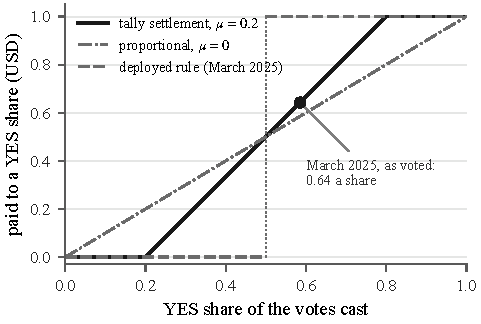
\includegraphics[width=0.98\columnwidth]{figures/fig_rule.pdf}
\caption{What a disputed question pays a Yes share as a function of Yes's share of the votes cast, for two answers and full participation. The deployed rule (threshold one half, as in March 2025) pays nothing or a dollar; with a third answer or abstentions, a vote that carries no answer past the threshold rolls and settles nothing. Proportional settlement~\cite{freeman2017} is the diagonal, and tally settlement with $\muparam = 0.2$ the sloped line. The circle is the March vote as cast.}
\label{fig:rule}
\end{figure}

\begin{table}[t]
\centering
\caption{Tally settlement replayed over every Polymarket vote that decided a payout, on the first round's tally; $\muparam = 0$ is proportional settlement. ``Below full'' is the share of the \rampYesNoBothPay{} Yes-or-No votes that both rules pay (\rampYesNoBothPayEraB{} in the 65\% era) whose winner is paid less than a dollar, and ``cut'' the median shortfall in cents. ``P10'' is the tenth percentile of the winner's payout in the \rampContestedSidedN{} contested Yes-or-No votes, ``10\%'' the most a tenth of the supply moves any payout in cents at full participation, and ``March'' the payout of the March 2025 ``Yes''.}
\label{tab:ramp}
\footnotesize
\setlength{\tabcolsep}{2.6pt}
\begin{tabular}{@{}ccccccc@{}}
\toprule
$\muparam$ & below full & 65\% era & cut & P10 & 10\% & March \\
\midrule
0 & \rampCutPctZero\% & \rampCutEraBPctZero\% & \rampHaircutZero & \rampWinnerPTenZero & \rampShiftTenPctZero & \rampMarchWithZero \\
0.10 & \rampCutPctTen\% & \rampCutEraBPctTen\% & \rampHaircutTen & \rampWinnerPTenTen & \rampShiftTenPctTen & \rampMarchWithTen \\
0.15 & \rampCutPctFifteen\% & \rampCutEraBPctFifteen\% & \rampHaircutFifteen & \rampWinnerPTenFifteen & \rampShiftTenPctFifteen & \rampMarchWithFifteen \\
0.20 & \rampCutPctTwenty\% & \rampCutEraBPctTwenty\% & \rampHaircutTwenty & \rampWinnerPTenTwenty & \rampShiftTenPctTwenty & \rampMarchWithTwenty \\
0.25 & \rampCutPctTwentyFive\% & \rampCutEraBPctTwentyFive\% & \rampHaircutTwentyFive & \rampWinnerPTenTwentyFive & \rampShiftTenPctTwentyFive & \rampMarchWithTwentyFive \\
0.30 & \rampCutPctThirty\% & \rampCutEraBPctThirty\% & \rampHaircutThirty & \rampWinnerPTenThirty & \rampShiftTenPctThirty & \rampMarchWithThirty \\
\bottomrule
\end{tabular}
\end{table}

\section{The March 2025 request, the slashing port and the counterfactuals}
\label{app:port}
\begin{table}[t]
\centering
\caption{The request that decided the minerals-deal market's payout (round 10085, second request), decoded from the voting contract, and the counterfactuals of the same arithmetic (UMA).}
\label{tab:march}
\footnotesize
\setlength{\tabcolsep}{3pt}
\begin{tabular}{@{}p{6.0cm}r@{}}
\toprule
Staked supply $S$ (UMA) & \marchStake \\
Threshold, $\theta = 50\%$ of $S$ & \marchStallStakedFifty \\
``Yes'' & \marchYes{} (\marchYesPct\%) \\
``Too early'' & \marchTooEarly{} (\marchTooEarlyPct\%) \\
``No'' & \marchNo \\
Did not vote & \marchAbstain{} (\marchAbstainPct\%) \\
Voters & \marchVoters \\
Three wallets, revealed 22:58 to 23:00 UTC & \marchWhale{} (\marchAlpha\%) \\
Margin of ``Yes'' over the threshold & \marchMargin{} (\marchMarginPct\%) \\
Stake the three wallets needed & \marchNeeded \\
Penalty pool, paid to ``Yes'' voters & \marchPool \\
\quad of which to the three wallets & \marchWhaleGain \\
Open interest when the round ended (USDC) & \marchOI \\
``Yes'' shares redeemed within a week (USDC) & \marchRedeemed \\
Pre-dispute 24-hour mean price of ``Yes'' & \marchTwap \\
\midrule
Stake they would have needed at $\theta = 65\%$ & \marchNeededSixtyFive \\
\quad shortfall at 65\% & \marchShortSixtyFive \\
Needed with the votes-cast denominator, 50\% & \marchNeededVotesCast \\
Blocking coalition, 65\% of staked & \marchStallStakedSixtyFive \\
Blocking coalition, 65\% of votes cast, rest voting its answer (Remark~\ref{rem:rest}) & \marchStallVotesSixtyFive \\
\bottomrule
\end{tabular}
\end{table}

\looseness=-1 The port reproduces \texttt{VotingV2}'s resolution test (total votes above the participation floor and modal votes above $\theta$ times the frozen supply) and its penalty arithmetic: the pool is $\lfloor(\lambda_n (S - v) + \lambda_w (v - v^{*}))/10^{18}\rfloor$, with $\lambda_n$ and $\lambda_w$ the contract's per-token penalties for not voting and for voting wrong ($0.1\%$ each, in its fixed-point units), a wrong or absent token pays $\lceil s\lambda / 10^{18}\rceil$, and a correct token receives $\lfloor s\cdot\text{pool}/v^{*}\rfloor$; the ceiling on penalties is the contract's \texttt{Math.ceilDiv}. Against the \portEvents{} penalty events emitted so far for each of the two March requests, every voter with an event matches to the wei (\portMatchedA{} and \portMatchedB{} voters, \portMismatched{} mismatches); the remaining events belong to absent stakers whose round stake is not in the vote events. The same arithmetic gives the counterfactuals in the lower part of Table~\ref{tab:march}.

\section{Captures of on-chain votes}
\label{app:delta}
\looseness=-1 For each capture we compute the governance token's abnormal log return against ETH over the week that starts on the day of the capture, from daily prices~\cite{defillama}, and scale it by the standard deviation of the token's overlapping weekly abnormal returns over the 365 days before. Beanstalk and Venus's VIP-42 lack a year of prices and are left out. Pooled, the captures that took nothing from their protocol show no significant mean loss; the one-sided 95\% bound on their mean weekly loss is \deltaBoundAllPct\%, or \deltaBoundWoPct\% without Indexed, whose token tripled against ETH that week. On each token's pre-event noise, a two-sided 5\% test detects a mean loss of \deltaDetectablePct\% four times in five. At the first group's median loss of \deltaDrainedMedianPct\%, the markets of \deltaUnprotectedAtDrainedMedian{} of the \rampMarkets{} contested payout votes remain beyond the rule's guarantee. Only one of the captures is of UMA's own vote; the others come from different protocols, successful and stopped captures are pooled, and a week's return against ETH does not isolate other news. For that one, UMA rose \econUmaOne\% in the day after the round closed while ETH fell \econEthOneAbs\%, outperformed ETH by \econAbnEthThree{} points over three days, and over the week fell \econUmaSevenAbs\% against ETH's \econEthSevenAbs\%, \econAbnEthSevenAbs{} points in log returns, less than half the standard deviation of its weekly return relative to ETH over the preceding year (\econSdEthSeven{} points); against BTC the weekly shortfall is \econAbnBtcSevenAbs{} points with a standard deviation of \econSdBtcSeven.

\begin{table}[t]
\centering
\caption{Captures and attempted captures of on-chain votes. Week: the governance token's simple abnormal return against ETH in the week from the capture; $z$: the log return over its standard deviation in the preceding 365 days; Took: whether the capture drained or diluted the protocol. $^{*}$One day: Curio's token was replaced the next day.}
\label{tab:delta}
\footnotesize
\setlength{\tabcolsep}{4pt}
\begin{tabular}{@{}lllcrr@{}}
\toprule
Capture & Token & Month & Took & Week & $z$ \\
\midrule
Build Finance & BUILD & 2022-02 & yes & $-99.7$\% & $-17.8$ \\
Audius & AUDIO & 2022-07 & yes & $-16.0$\% & $-1.0$ \\
Mango Markets & MNGO & 2022-10 & yes & $-41.2$\% & $-4.7$ \\
Tornado Cash & TORN & 2023-05 & yes & $-34.5$\% & $-2.4$ \\
Synthetify & SNY & 2023-10 & yes & $-7.1$\% & $-0.3$ \\
Curio & CGT & 2024-03 & yes & $-11.8$\%$^{*}$ & $-0.6$ \\
\midrule
Steem & STEEM & 2020-03 & no & $+19.8$\% & $+1.9$ \\
Maker flash vote & MKR & 2020-10 & no & $-4.7$\% & $-0.5$ \\
Curve, Mochi & CRV & 2021-11 & no & $+15.6$\% & $+0.7$ \\
Compound TUSD & COMP & 2022-02 & no & $-6.8$\% & $-0.6$ \\
Yam & YAM & 2022-07 & no & $-14.0$\% & $-1.1$ \\
Indexed & NDX & 2023-11 & no & $+204.1$\% & $+3.9$ \\
Compound 289 & COMP & 2024-07 & no & $-3.8$\% & $-0.5$ \\
UMA & UMA & 2025-03 & no & $-5.5$\% & $-0.5$ \\
\bottomrule

\end{tabular}
\end{table}

\section{Five resolution designs}
\label{app:deployments}
Table~\ref{tab:deployments} places the designs of Section~\ref{sec:related} and Bittensor's Yuma consensus in the frame of Theorem~\ref{thm:tally}.

\begin{table}[t]
\centering
\caption{Resolution designs and their position relative to the class of resolve-or-roll rules.}
\label{tab:deployments}
\footnotesize
\setlength{\tabcolsep}{1.5pt}
\begin{tabular}{@{}p{1.45cm}p{3.8cm}p{3.05cm}@{}}
\toprule
Design & Rule & In the class? \\
\midrule
UMA DVM 2.0 & modal answer $> 65\%$ of staked, else roll; deleted after 4 rolls & yes; block $35\% - \hF$, by abstaining \\
same, votes cast & modal answer $> 65\%$ of votes cast & yes; block $35\% - \hF$, by voting \\
Kleros & plurality of a stake-drawn jury; appeals with $2n+1$ jurors; incoherent jurors pay coherent ones & one round yes ($\theta_f = 1/2$); the appeal ladder no \\
Augur v2 & escalating REP bonds; a bond of 2.5\% of REP forks the token & no: bonds, not tallies; the terminal is a fork \\
Reality.eth & doubling bonds, timeout, designated arbitrator & no: bonds and an arbitrator \\
Bittensor Yuma & stake-weighted median of validator weights & yes; no roll; $\theta_f = 1/2$ \\
\bottomrule
\end{tabular}
\end{table}

\end{document}
